
\def\anon{0} %% set to 1 for anonymous submissions, hides acknowledgements and author names
\def\full{1} %% set to 0 for springer proceedings


\ifnum\full=1
\documentclass[11pt]{llncs}


\addtolength{\parskip}{1pt}
\else
\documentclass[10pt, runningheads]{llncs}
\usepackage{times}

\fi




\usepackage{makeidx}
\usepackage[dvips]{graphicx}
\usepackage{graphicx}

\usepackage{comment}

\usepackage{listings}
\usepackage[mathscr]{eucal}
\usepackage{bm}
\usepackage{array}
\usepackage{url}
\usepackage{calc}
\usepackage{float}
\usepackage{latexsym}
\usepackage{rotating}
\DeclareGraphicsExtensions{.eps,.jpg,.png,.pdf}
%\usepackage[usenames, dvipsnames]{xcolor}
\usepackage[dvipsnames]{xcolor}
\usepackage[sort,nocompress]{cite}
\usepackage{colortbl}
\usepackage{multirow}
\usepackage{lscape}
\usepackage{amsmath}
\let\proof\relax
\let\endproof\relax
\usepackage{amsthm,amsfonts,amssymb}
\usepackage{hyperref}
\usepackage{pdflscape}


%\usepackage{natbib}

\def\rmdefault{ptm}

\usepackage{setspace}
\usepackage{color}
\ifnum\full=1
\usepackage[margin=0.9in]{geometry}
\usepackage{fullpage}

\setlength{\parskip}{0cm}

%\setstretch{1.03}
%\addtolength{\parskip}{1pt}
\setcounter{page}{0}
\renewcommand{\tabcolsep}{5pt}
\else
\renewcommand{\tabcolsep}{0pt}
\fi

\renewcommand{\arraystretch}{1.2}

\hyphenpenalty=5000
\tolerance=1000




%\ifnum\full=1
%\usepackage{natbib}
%\bibliographystyle{alpha}
%\setlength{\bibsep}{0pt}
%\renewcommand{\bibsection}{\section*{References}\small}
%\else
%\usepackage[numbers]{natbib}
%\bibliographystyle{splncs04}
%\fi



\DeclareMathOperator{\Exp}{E}
\DeclareMathOperator{\Var}{Var}
\DeclareMathOperator{\poly}{poly}
\DeclareMathOperator{\Supp}{Supp}

\usepackage{enumitem}


\usepackage{tikz}
\usetikzlibrary{arrows,shapes}
\usetikzlibrary{plotmarks}


%notes

%\definecolor{myorange}{rgb}{0.99,0.6,0.25}
%\newcommand{\pmnote}[1]{\colorbox{myorange}{\parbox{0.9\linewidth}{[{\footnotesize {\bf PM:} { {#1}}}]}}}


\definecolor{mycolor}{rgb}{0.75,0.95,0.05}
\newcommand{\pmnote}[1]{\colorbox{mycolor}{\parbox{0.9\linewidth}{[{\footnotesize {\bf PM:} { {#1}}}]}}}

\newcommand{\tsnote}[1]{\colorbox{orange}{\footnotesize\color{white}\textbf{TS: }#1}}

\definecolor{unmellowyellow}{rgb}{1.0, 1.0, 0.4}
\newcommand{\agnote}[1]{\colorbox{unmellowyellow}{\parbox{0.9\linewidth}{[{\footnotesize {\bf AG:} { {#1}}}]}}}
%% Sets

\newcommand{\Z}{\mathbb{Z}}
\newcommand{\N}{\mathbb{N}}
\newcommand{\R}{\mathbb{R}}
\newcommand{\C}{\mathbb{C}}
\newcommand{\F}{\mathbb{F}}
\newcommand{\Znm}{\mathbb{Z}_q^{n \times m}}

%matrices
\newcommand{\matzero}{\mathbf{0}}
\newcommand{\matA}{\mathbf{A}}
\newcommand{\matB}{\mathbf{B}}
\newcommand{\matC}{\mathbf{C}}
\newcommand{\matE}{\mathbf{E}}
\newcommand{\matF}{\mathbf{F}}
\newcommand{\matG}{\mathbf{G}}
\newcommand{\matI}{\mathbf{I}}
\newcommand{\matM}{\mathbf{M}}
\newcommand{\matP}{\mathbf{P}}
\newcommand{\matR}{\mathbf{R}}
\newcommand{\matS}{\mathbf{S}}
\newcommand{\matT}{\mathbf{T}}
\newcommand{\matU}{\mathbf{U}}
\newcommand{\matV}{\mathbf{V}}
\newcommand{\matW}{\mathbf{W}}
\newcommand{\matX}{\mathbf{X}}
\newcommand{\matY}{\mathbf{Y}}
\newcommand{\matZ}{\mathbf{Z}}


%vectors
\newcommand{\veca}{\mathbf{a}}
\newcommand{\vecb}{\mathbf{b}}
\newcommand{\vecc}{\mathbf{c}}
\newcommand{\vecd}{\mathbf{d}}
\newcommand{\vece}{\mathbf{e}}
\newcommand{\veci}{\mathbf{i}}
\newcommand{\vecj}{\mathbf{j}}
\newcommand{\veck}{\mathbf{k}}
\newcommand{\vecl}{\mathbf{l}}
\newcommand{\vecm}{\mathbf{m}}
\newcommand{\vecp}{\mathbf{p}}
\newcommand{\vecr}{\mathbf{r}}
\newcommand{\vecs}{\mathbf{s}}
\newcommand{\vecv}{\mathbf{v}}
\newcommand{\vecw}{\mathbf{w}}
\newcommand{\vecu}{\mathbf{u}}
\newcommand{\vecx}{\mathbf{x}}
\newcommand{\vecy}{\mathbf{y}}
\newcommand{\vecz}{\mathbf{z}}





%FiLIP notations

\newcommand{\FLIP}{\textsf{FLIP}}
\newcommand{\IFPl}{\text{Improved Filter Permutator} }
\newcommand{\IFPs}{\text{IFP} }

\newcommand{\FiLIP}{\textsf{FiLIP}}
\newcommand{\FiLIPDSM}{\mathsf{FiLIP}_{\mathsf{DSM}}}
\newcommand{\FiLIPXMAJ}{\mathsf{FiLIP}_{\mathsf{XMAJ}}}

%Boolean functions

\newcommand{\Bfn}[1]{\mathcal{B}_{#1}}
\newcommand{\BN}{\mathcal{B}_n}
\newcommand{\Bn}[1]{\mathcal{B}_{#1}}
\newcommand{\Bnstar}[1]{\mathcal{B}_{#1}^*}

\newcommand{\Bvad}[3]{\mathcal{B}({#1},{#2},{#3})}


\newcommand{\AI}{\mathsf{AI}}
\newcommand{\AN}{\mathsf{AN}}
%\newcommand{\difAN}[1]{\Delta_{\mathsf{AN}}(#1)}
%\newcommand{\DAN}{\mathsf{d}\mathsf{AN}}
%\newcommand{\Sd}{\mathsf{S}_\mathsf{d}}
\newcommand{\SD}{\mathsf{SD}}
\newcommand{\FAI}{\mathsf{FAI}}
\newcommand{\NL}{\mathsf{NL}}
\newcommand{\NLk}[1]{\mathsf{NL}_{#1}}
%\newcommand{\NLd}{\mathsf{NL_d}}
\newcommand{\res}{\mathsf{res}}
\newcommand{\bal}{\mathsf{bal}}
\newcommand{\gnlk}{\mathsf{GWNL}}


\newcommand{\DS}[1]{\mathsf{DS}(#1)}
\newcommand{\DSR}[2]{\mathsf{DS}^{#2}(#1)}
%\newcommand{\matAI}[3]{\mathbf{A}_{#2,#3}(#1)}

\newcommand{\WPB}[1]{\mathcal{WPB}_{#1}}
\newcommand{\WAPB}[1]{\mathcal{WAPB}_{#1}}
\newcommand{\SWAPB}[1]{\mathcal{SWAPB}_{#1}}
\newcommand{\SYM}[1]{\mathcal{SYM}_{#1}}
%for affine weightwise: degree and number of variables
\newcommand{\WD}[2]{\mathcal{WD}^{#1}_{#2}}
\newcommand{\Ekn}[2]{\mathsf{E}_{#1,#2}}
\newcommand{\Code}[2]{\mathsf{P}_{#1,#2}}
\newcommand{\mdist}[2]{\mathsf{d}_{#1,#2}}
%\newcommand{\Dka}[2]{\mathsf{D}_{#1}(#2)}
\newcommand{\Dnka}[3]{\mathsf{D}_{#1,#2}(#3)}

\newcommand{\dis}{\mathsf{c_1}}




\newcommand{\mnlk}[2]{\mu_{#1,#2}}
\newcommand{\Mnlk}[2]{\mathsf{M}_{#1,#2}}
\newcommand{\mnl}[1]{\mu_{#1}}
\newcommand{\Mnl}[1]{\mathsf{M}_{#1}}

\newcommand{\DistWkn}[2]{\mathfrak{W}_{#1,#2}}
\newcommand{\DistWn}[1]{\mathfrak{W}_{#1}}
\newcommand{\Dkn}[2]{\mathfrak{D}_{#1,#2}}
\newcommand{\Dn}[1]{\mathfrak{D}_{#1}}

\newcommand{\kraw}[3]{\mathsf{K}_{#1}(#2,#3)}
\newcommand{\phikn}[2]{\varphi_{#1,#2}}

\newcommand{\const}[2]{g_{#1,#2}}
\newcommand{\setn}[1]{S_{#1}}
\newcommand{\symsetsmall}[1]{A_{#1}}
\newcommand{\symset}[2]{B_{#1,#2}}


%usual notations
\newcommand{\supp}{\mathsf{supp}}
\newcommand{\suppk}[1]{\mathsf{supp}_{#1}}
\newcommand{\w}{\mathsf{w_H}}
\newcommand{\hd}{\mathsf{d_H}}
\newcommand{\degg}{\mathsf{deg}}
\newcommand{\Span}{\mathsf{Span}}
\newcommand{\rank}{\mathsf{rank}}
%Walsh transform
\newcommand{\wt}[1]{\mathcal W_{#1}} 
\newcommand{\Wsupp}[1]{\mathsf{Wsupp}_{#1}} 
%restricted Walsh transform W_k,a (f)
\newcommand{\wtk}[2]{\mathcal{W}_{#1,#2}} 

%S-equivalent classes
\newcommand{\sclass}[1]{\mathcal{S}(#1)}


\newcommand{\set}[1]{\left\{#1\right\}}
\newcommand{\mAN}[1]{\mathsf{d}_{#1}}


%gates
\newcommand{\AND}{\textsf{AND}}
\newcommand{\XOR}{\textsf{XOR}}
\newcommand{\MUX}{\textsf{MUX}}


%families of functions
\newcommand{\MAJ}{\textsf{MAJ}}
\newcommand{\DSM}{\textsf{DSM}}
\newcommand{\XORTHR}{\textsf{XOR-THR}}
\newcommand{\XORMAJ}{\textsf{XOR-MAJ}}

\newcommand{\xorlk}[2]{{\mathsf{XOR}}_{#1}  \mathsf{M}_{#2}} 
\newcommand{\xormaj}[2]{{\mathsf{XOR}}_{#1}  \mathsf{MAJ}_{#2}} 
%\newcommand{\xorthr}[3]{{\mathsf{XOR}}_{#1}  \mathsf{T}_{{#2},{#3}}} 
\newcommand{\xorthr}[3]{{\mathsf{XOR}}_{#1}+\mathsf{T}_{{#2},{#3}}}
\newcommand{\tri}[1]{{T}_{#1}}
\newcommand{\thr}[2]{\mathsf{T}_{{#1},{#2}}}
\newcommand{\xor}[1]{\mathsf{XOR}_{#1}}
\newcommand{\maj}[1]{\mathsf{MAJ}_{#1}}


\newcommand{\nbf}[1]{\mathsf{C}_{#1}}
\newcommand{\nbfodd}[2]{\mathsf{A}_{#1,#2}}
\newcommand{\nbfeven}[2]{\mathsf{B}_{#1,#2}}

%direct sum vector and simplified value vector
\newcommand{\dsv}[1]{\mathbf{m}_{#1}}
\newcommand{\svv}[1]{\mathbf{s}_{#1}}

% Define a custom theorem style for bold optional arguments
\newtheoremstyle{boldoptional} % Name of the style
  {3pt}                        % Space above
  {3pt}                        % Space below
  {\itshape}                   % Body font
  {}                           % Indent amount
  {\bfseries}                  % Theorem head font
  {.}                          % Punctuation after theorem head
  { }                          % Space after theorem head
  {\thmname{#1}\thmnumber{ #2}\thmnote{ (\textbf{#3})}} % Bold optional argument

% Apply the new style to Property
\theoremstyle{boldoptional}
\newtheorem{Prop}{Property}
\newtheorem{Cons}{Construction}


% For algorithms
\usepackage{algorithm,algpseudocode}

\renewcommand{\algorithmicrequire}{\textbf{Input:}}
\renewcommand{\algorithmicensure}{\textbf{Output:}}
% \renewcommand{\ALG@name}{Construction}
\newenvironment{constr}[1][htb]{%
\floatname{algorithm}{Construction}% Update algorithm name
   \begin{algorithm}[#1]%
  }{\end{algorithm}}
 
\algnewcommand\algorithmicparfor{\textbf{par-for}}
\algdef{S}[FOR]{ParFor}[1]{\algorithmicparfor\ #1\ \algorithmicdo}
 
%latin

\newcommand{\ie}{\textit{i.e.}}
\newcommand{\eg}{\textit{e.g.}}
\newcommand{\ea}{\textit{et al.}}

%Tim's stuff
\newtheorem{Corollary}{Corollary}
\newcommand{\ii}{\mathrm i\mkern1mu} %Imaginary unit
\newcommand{\ee}{\mathrm e\mkern1mu} %Euler constant
\newcommand{\dd}{\,\mathrm d} %Differential
\newcommand{\ui}[1]{^{(#1)}} %Upper index
\newcommand{\mycomment}[1]{} %Comment out entire parts
\usepackage{mleftright}
\mleftright %Less space when using \left and \right


\newcommand{\tablecaption}[1]{%
   \vspace{3pt} % Adds space above the caption
   \caption{#1} % Displays the caption text
}

\let\leq=\leqslant %Replace symbol for \leq
\let\geq=\geqslant %Replace symbol for \geq

\newcommand{\hwbf}{\textsf{HWBF}}

%No line break before lists
\makeatletter
\@beginparpenalty=10000
\makeatother


\begin{document}
	\title{Revisited hidden weight bit function}

	
	\titlerunning{Revisited Hidden weight bit function}
\author{
	Pierrick M\'eaux\inst{1},
	Tim Seuré\inst{1}, 
	Deng Tang\inst{2}
%	Pierrick M\'eaux\orcidID{0000-0001-5733-4341}\inst{1},
%	Tim Seuré\inst{1}, 
%	Deng Tang\orcidID{0000-0002-8373-9200}\inst{2}
}
\authorrunning{P. M\'eaux, T. Seuré, D. Tang}

	
\institute{
	University of Luxembourg, Luxembourg\\ \email{pierrick.meaux@uni.lu, tim.seure@uni.lu} 
	%\and
%		University of Luxembourg, Luxembourg\\ \email{pierrick.meaux@uni.lu}
	\and
	Shanghai Jiao Tong University, Shanghai, China.\\
	\email{dengtang@sjtu.edu.cn}
}

	
	
	
	%----------------------------------------------------------------
	\maketitle


\institute{
	University of Luxembourg, Luxembourg\\
	\email{pierrick.meaux@uni.lu}		
}	
	
	\begin{abstract}
	
		
	\end{abstract}


\section{Introduction}

\pmnote{short intro:

HWBF introduced in x, interesting for its cryptographic criteria and easy implementation. cryptographic properties studied in y such as balancedness, algebraic immunity and nonlinearity. 
New potential uses in a stream cipher, or modifications. Use: transciphering and works aiming at finding Boolean functions easy to evaluate homomorphically, input oblivious algorithms. 
Nonlinearity a bit low for direct use.



Contributions: new function as addition of HWBF and quadratic bent function. We show when the function is balanced, formalize and study its nonlinearity. Bounds on the nonlinearity of $f$, generalization to a family of function, and an algorithm for estimating the nonlinearity for $n$ up to $80$. Comparisons with other functions and practical values of the parameters for $n$ up to $20$.



}





\section{Preliminaries}

For $v$ a binary vector of length $n$ we denote by $\w(v)$ its Hamming weight: $\w(v)=|\{i\in [1,n] \, | \, x_i=1\}|$.

\pmnote{Preliminaries to adapt}


\subsection{Boolean functions and cryptographic parameters}

In this part we recall general concepts on Boolean functions and their cryptographic properties we use in this article. 
For a deeper introduction on Boolean functions and their cryptographic parameters we refer to the book~\cite{Carlet20} and to~\cite{TOSC:CarMeaRot17} for the weightwise properties, also called properties on the slices.
For $k \in [0,n]$ we denote $\Ekn{k}{n}$ the set $\{x\in \F_2^n \, | \, \w(x)=k  \}$ and call it slice of the Boolean hypercube (of dimension $n$). 

%Accordingly, the Boolean hypercube is partitioned into $n+1$ slices where the elements have the same Hamming weight.

\begin{definition}[Boolean Function]\label{def:bool_f}
	A Boolean function $f$ in $n$ variables is a function from $\F_2^n$ to $\F_2$. 
	The set of all Boolean functions in $n$ variables is denoted by $\BN$, and we denote $\BN^*$ the set without the null function.
\end{definition}


\begin{definition}[Balancedness]\label{def:balancedness}
	A Boolean function $f\in \BN$ is called balanced if $|\supp(f)|=2^{n-1}=|\supp(f+1)|$. 
	
%	For $k\in [0,n]$ the function is said balanced on the slice $k$ if $||\suppk{k}(f)|-|\suppk{k}(f+1)| |\le 1$. In particular when $|\Ekn{k}{n}|$ is even $|\suppk{k}(f)|=|\suppk{k}(f+1)|=|\Ekn{k}{n}|/2$.
\end{definition}

\begin{definition}[Algebraic Normal Form (ANF) and degree]\label{def:anf}
	We call Algebraic Normal Form of a Boolean function $f$ its $n$-variable polynomial representation over $\F_2$ (\textit{i.e.} belonging to $\F_2[x_1,\dots,x_n]/(x_1^2+x_1,\dots,x_n^2+x_n)$):
	\[f(x_1,\dots,x_n)= \sum_{I \subseteq [1,n]} a_I \left( \prod_{i \in I} x_i \right) \]%x_1,\dots,x_n=\sum_{I \subseteq [1,n]} a_I x^I,\]
	where $a_I\in \F_2$. 	
	The (algebraic) degree of $f$, denoted $\degg(f)$ is: \[\degg(f)=\
	\max_{I\subseteq [1,n]}\{ |I|\, | \, a_I=1\}  \text{ if $f$ is not null},0  \text{ otherwise}.\]
\end{definition}




\begin{definition}[Walsh transform and restricted Walsh transform]\label{def:walsh_transform}
	Let $f\in \Bn{n}$ be a Boolean function, its Walsh transform $\wt{f}$ at $a \in \F_2^n$ is defined as:
	\[  \wt{f} (a) = \sum_{x \in \F_2^n} (-1)^{f(x) +  a \cdot x }.\]
	%	The Walsh support is the set $\Wsupp{f}=\{ a\in \F_2^n\, | \, \wt{f} (a) \neq 0 \}$.
	Let $f\in \Bn{n}$, $S \subset \F_2^n$, its Walsh transform restricted to $S$ at $a \in \F_2^n$ is defined as:
	\[  \wt{f,S} (a) = \sum_{x\in S} (-1)^{f(x)+a \cdot x}.\]
	For $S=\Ekn{k}{n}$ we denote $\wt{f,\Ekn{k}{n}} (a)$ by $\wtk{f}{k}(a)$.%, and for $a= 0_{n}$ we denote $\wtk{f}{k}(a)$ as $\wtk{f}{k}(0)$.
\end{definition}


	


%\begin{definition}[Algebraic Immunity] \label{def:ai}
%	The algebraic immunity of a Boolean function $f\in \Bfn{n}$, denoted as $\AI(f)$, is defined as:
%	\[ \AI(f) = \min_{g \neq 0}\{ \degg(g) \; | \; fg = 0 \; \text{or} \; (f + 1)g = 0 \}{,} \]
%	where $\degg(g)$ is the algebraic degree of $g$.
%	The function $g$ is called an annihilator of $f$ (or $f + 1$). 
%	Additionally we denote $\AN(f) = \min_{g \neq 0}\{ \degg(g) \; | \; fg = 0\}$.
%\end{definition}
\begin{definition}[Nonlinearity]%and weightwise nonlinearity
	\label{def:nl}
	The nonlinearity $\NL(f)$ of a Boolean function $f\in \BN$, where $n$ is a positive integer, is the minimum Hamming distance between $f$ and all the affine functions in $\BN$:
	\[ \NL(f) = \min_{g,\, \degg(g)\leq 1} \{ \hd(f,g) \}{,} \]
	where $g(x)=a\cdot x+\varepsilon$, $a\in \F_2^n, \varepsilon\in \F_2$. 	
	The nonlinearity can also be defined from the Walsh transform:
	\[ \NL(f) = 2^{n-1}- \frac{1}{2} \max_{a\in \F_2^n}{|\wt{f}(a)|}. \]
\end{definition}

When $n$ is even, the nonlinearity of a function can reach at most $2^{n-1}-2^{n/2 -1}$. Functions reaching this maximum are called bent functions. The quadratic function $d_n$ given by: $d_n(x)=\sum_{i \text{ odd}}^n x_i x_{i+1}$ is an example of bent function.






\begin{definition}[Algebraic immunity] \label{def:ai}
	The algebraic immunity of a Boolean function $f\in \Bfn{n}$, denoted as $\AI(f)$, is defined as:
	\[ \AI(f) = \min_{g \neq 0}\{ \degg(g) \; | \; fg = 0 \; \text{or} \; (f + 1)g = 0 \}{,} \]
	where $\degg(g)$ is the algebraic degree of $g$.
	The function $g$ is called an annihilator of $f$ (or $f + 1$). 
\end{definition}

\subsection{Symmetric Functions, HWBF and weightwise degree-d functions}




The $n$-variable \emph{Boolean symmetric functions} are those that are constant on each slice $\Ekn{k}{n}$ for $k\in [0,n]$. 
This class has been assiduously studied in the context of cryptography, see \eg \cite{IEEE:Carlet04,IEEE:CanVid05,INDO:BraPre05,DM:SarMai07,IEEE:QFLW09,IEEE:CheLu11,Latin:Meaux19,CCDS:Meaux21,IEEE:CarMea21}.
In this article we mainly consider the slice indicator functions and the majority functions.
%\begin{definition}[Elementary symmetric functions]
%Let $i\in [0,n]$, the elementary symmetric function of degree $i$ in $n$ variables, denoted $\sigma_{i,n}$, is the function which ANF contains all monomials of degree $i$ and no monomials of other degrees. 
%\end{definition}
\begin{definition}[Slice indicator functions]\label{def:slice}
 Let $k\in [0,n]$, the indicator function of the slice of weight $k$ is defined as:
 \[\forall  x\in \mathbb{F}_2^{n}, \quad \phikn{k}{n}(x) = 1 \text{ if and only if } \w(x) = k.\]
\end{definition}


\begin{definition}[Majority function]\label{def:maj}
    The \emph{majority function} in $n$ variables is the Boolean function $\textsf{Maj}\in\BN$ defined as:
    \[
        \textsf{Maj}(x)=0\iff\w(x)<n/2.
    \]
\end{definition}

Bigger families of functions can be obtained by considering functions of bounded degree on each slice, it corresponds to the concept of weightwise degree-$d$ function introduced in~\cite{DAM:GinMea22} for $d=1$ and~\cite{DAM:MeaOza24} for the general case. 

\begin{definition}[Weightwise degree-$d$ functions (~\cite{DAM:MeaOza24} Definition 12)]\label{def:wwdegd}
	Let $n\in \N^*$ and for $k\in[0,n]$ $\phikn{k}{n}$ denotes the indicator function of $\Ekn{k}{n}$. 
	An $n$-variable Boolean function $f$, written as $f=\sum_{k=0}^n f_k \phikn{k}{n}$, is called weightwise degree-$d$ if and only if for each $k\in [0,n]$ $f_k$ coincide with a function of degree at most $d$ over $\Ekn{k}{n}$. 
		The set of weightwise degree-$d$ functions is denoted by $\WD{d}{n}$.
		
Additionally, a weightwise degree-$d$ function is called cyclic weightwise degree-$d$ function if for all $i\in [1,n]$ it holds $f_i(x)=f_0(O^i(x))$, where $O^i$ denotes the cyclic shift by $i$ positions, $O^i(x_1,\dots,x_n)=(x_{1+i \mod n},\dots,x_{n+i \mod n})$, the representative modulo being taken as an integer between $1$ and $n$.
\end{definition}



Various weightwise affine functions (\ie belonging to $\WD{1}{n}$) have been exhibited such as in~\cite{TOSC:CarMeaRot17} where the bent functions in Propositions $1$ and $2$ are weightwise affine or in~\cite{DAM:GinMea22} to show than no weightwise perfectly balanced function is weightwise affine for $n\ge 8$. 
The most known example of weightwise affine function is the hidden weight bit function introduced in~\cite{IEEE:Bryant91}, the one obtained by fixing $f_0=0$ and $f_k=x_k$ for $k \in [n]$. The cryptographic properties of this function have been studied in~\cite{DAM:WCST14}, showing good algebraic properties for this function.

\begin{definition}[Hidden Weight Bit Function (HWBF)]\label{def:hwbf}
	For $n\in \N^*$, we call Hidden Weight Bit Function (HWBF) the $n$-variable Boolean function defined by:
	\[h(x)= \left\{ 
	\begin{array}{l l}
	0 & \quad \text{ if } \w(x) =0, \\
	x_k & \quad \text{ if } \w(x)=k.
	\end{array} \right. \] 

\end{definition}

In~\cite{DAM:MeaOza24}, the parameters of different functions from $\WD{1}{n}$ and $\WD{2}{n}$ are studied experimentally for $n$ up to $20$ and lower bounds are given for the nonlinearity for all $n$. 
These bounds focus on cyclic weightwise quadratic functions and involve sums of binomial coefficients. For simplicity, in the following we provide only the nonlinearity values of the majority function and HWBF, as these bounds will be used for comparison.


%We summarize the known results on the cryptographic criteria of weightwise affine functions we will use in this article in the following property.


%\pmnote{complete the following prop. Choose between nonlinearity or $\max_{a\in\mathbb F_2^n}|\wt f(a)|$ \color{blue} Tim: I started, but please do the remaining two items.}
\iffalse
\begin{Prop}[Nonlinearity of some functions from $\WD{1}{n}$, \cite{DCC:DalMaiSar06,DAM:WCST14,DAM:MeaOza24}\label{prop:wwd1}]
Let $n\in \N^*$ even, the following hold for functions in $\WD{2}{n}$. 
\begin{itemize}
    \item The majority function $f\in\WD{2}{n}$ introduced in Definition~\ref{def:maj} satisfies:
    \[
        \NL(f)=2^{n-1}-\binom{n-1}{\frac n2}.
    \]
    \item The HWBF $f\in\WD{2}{n}$ introduced in Definition~\ref{def:hwbf} satisfies:
    \[
        \NL(f)=2^{n-1}-2\binom{n-2}{\frac{n-2}{2}}.
    \]
	\item  bound for the cyclic weightwise linear (adapt Theorem 1 of \cite{DAM:MeaOza24})
	\item  bound for the cyclic weightwise quadratic function $t$  (adapt Theorem 2 of \cite{DAM:MeaOza24})
\end{itemize}
\end{Prop}
\fi 

\begin{Prop}[Nonlinearity of some functions from $\WD{1}{n}$\label{prop:wwd1}]
Let $n\in \N^*$ even, the following hold for the following functions in $\WD{1}{n}$: 
\begin{itemize}
	\item (\eg ~\cite{DCC:DalMaiSar06}, Theorem $3$) The majority function $\textsf{Maj}_n$ introduced in Definition~\ref{def:maj} satisfies:
	\[
	\NL(\textsf{Maj}_n)=2^{n-1}-\binom{n-1}{\frac n2}.
	\]
	\item (\cite{DAM:WCST14}, Theorem $3$) The HWBF $h$ introduced in Definition~\ref{def:hwbf} satisfies:
	\[
	\NL(h)=2^{n-1}-2\binom{n-2}{\frac{n-2}{2}}.
	\]	
\end{itemize}
\end{Prop}






\subsection{Krawtchouk polynomials}
We use Krawtchouk polynomials and some of their properties to prove one of our results, we give the necessary preliminaries here and refer to \eg ~\cite{book:MacSlo78} for more details.

\begin{definition}[Krawtchouk Polynomials]\label{def:Kraw}
	The Krawtchouk polynomial of degree $k$, with $0\leq k\leq n$ is given by: $ \displaystyle \kraw{k}{\ell}{n}=\sum_{j=0}^{k} (-1)^j \binom{\ell}{j} \binom{n-\ell}{k-j}$. 
	
	Krawtchouk polynomials are characterized by the generating series: $ \displaystyle (1+z)^{n-x} (1-z)^x=\sum_{k=0}^\infty \kraw{k}{x}{n} z^k$.
\end{definition}






\section{Revisited HWBF and balancedness}
%\subsection{Restricted Walsh transform of $f$ in a recursive fashion}

In this part we formally define the revisited HWBF function $f$ and introduce a quantity that allows us to study its balancedness and nonlinearity.

\begin{definition}[Revisited HWBF]\label{def:revHWBF}
Let $n\in \N^*$, even, we call revisited HWBF and denote by $f$ the Boolean function defined as:
\[f(x_1,\cdots,x_n)=\left(\sum_{i=1}^{n/2} (x_i+1) x_{i+\frac{n}{2}}\right) + \sum_{k=1}^n \phikn{k}{n} x_k.\]
\end{definition}


%We study the function $f$ in an even number of variables $n$ defined as the following:
%\[f(x_1,\cdots,x_n)=\left(\sum_{i=1}^{n/2} (x_i+1) x_{i+\frac{n}{2}}\right) + \sum_{k=1}^n \phikn{k}{n} x_k.\]

Since $f$ is the sum of a quadratic function and a weightweise affine function, it is a weightwise quadratic function. 
Using the formalism of Definition~\ref{def:wwdegd} $f$ is the WWQ function defined by:% $f_0=0$ and for $k\in [1,n]$ $f_k=x_k + \sum_{i=1}^{n/2} (x_i+1) x_{i+n/2}$.
\[f_0=0, \quad \text{ and } \quad \forall k \in [1,n], \, f_k=x_k+\sum_{i=1}^{n/2} (x_i+1) x_{i+\frac{n}{2}}.\]

This form allows to derive the restricted Walsh transform of $f$, which can be a useful tool to study the balancedness and bound the nonlinearity of a function.
%Maybe add examples, such as OM24, M24



%We study the restricted Walsh transform  of $f$ to bound its nonlinearity.
\begin{proposition}\label{prop:restrWT}
Let $n \in \N^*$ even, and $f$ be the function from Definition~\ref{def:revHWBF}, for all $k\in [0,n]$ its restricted Walsh transform in $a\in \F_2^n$ is given by:
\[\wtk{f}{k}(a)=\sum_{x \in \Ekn{k}{n}} (-1)^{\sum_{i=1}^{n/2} x_i x_{i+\frac{n}{2}}+ c \cdot x},\]
where $c$ is the $n$-length binary vector such that $c=a+e_k+\sum_{i=n/2+1}^n e_i$ where the $e_i$ denotes the canonical vector with $1$ in position $i$.
\end{proposition}
\begin{proof}
%\begin{align*}
%	\wtk{f}{k}(a)&=\sum_{x \in \Ekn{k}{n}} (-1)^{f(x)+a \cdot x}
%	=\sum_{x \in \Ekn{k}{n}} (-1)^{x_k + \sum_{i=1}^{n/2} (x_i+1) x_{i+\frac{n}{2}}+ a \cdot x}\\
%	&=\sum_{x \in \Ekn{k}{n}} (-1)^{\sum_{i=1}^{n/2} x_i x_{i+\frac{n}{2}}+ c \cdot x},
%\end{align*}
%\begin{align*}
\[	\wtk{f}{k}(a)=\sum_{x \in \Ekn{k}{n}} (-1)^{f(x)+a \cdot x}
	=\sum_{x \in \Ekn{k}{n}} (-1)^{x_k + \sum_{i=1}^{n/2} (x_i+1) x_{i+\frac{n}{2}}+ a \cdot x}\\
	=\sum_{x \in \Ekn{k}{n}} (-1)^{\sum_{i=1}^{n/2} x_i x_{i+\frac{n}{2}}+ c \cdot x},\]
where $c$ denotes the $n$-length binary vector such that $c=a+e_k+\sum_{i=n/2+1}^n e_i$ and $e_i$ denotes the $i$-th canonical vector.
\end{proof}

%\begin{align*}
%\wtk{f}{k}(a)&=\sum_{x \in \Ekn{k}{n}} (-1)^{f(x)+ax}\\
%&=\sum_{x \in \Ekn{k}{n}} (-1)^{x_k + \sum_{i=1}^{n/2} (x_i+1) x_{i+\frac{n}{2}}+ ax}\\
%&=\sum_{x \in \Ekn{k}{n}} (-1)^{\sum_{i=1}^{n/2} x_i x_{i+\frac{n}{2}}+ (c)x},
%\end{align*}
%where $c$ is the $n$-length binary vector such that $c=a+e_k+\sum_{i=n/2+1}^n e_i$ where the $e_i$ denotes the canonical vector with "1" in position $i$.

Accordingly, we can study the restricted Walsh transform of this function by analyzing the one of $\sum_{i=1}^{n/2} x_i x_{i+\frac{n}{2}}$, for all $a$. We introduce the following notations.

\begin{definition}
Let $n\in \N$ be an even number, and $a\in \F_2^n$. We denote $d_n$ the function given by: $d_n(x)=\sum_{i \text{ odd}}^n x_i x_{i+1}$, 
and we denote by $\Dnka{n}{k}{a}$ the quantity:
\[\Dnka{n}{k}{a}= \sum_{x\in \Ekn{k}{n}} (-1)^{d_n(x) +a x}\]
\end{definition}

We can give a recursive relation for $\Dnka{n}{k}{a}$.




\begin{proposition}\label{prop:recursiveDnka}
Let $n\in \N$ be an even number, $k$ an integer in the range $[0,n]$ and $a\in \F_2^n$. the Following holds on $\Dnka{n}{k}{a}$:
\begin{itemize}
	\item For $n=0$, $\Dnka{0}{k}{a}=1$ if $k=0$ and $\Dnka 0ka=0$ otherwise.
	\item if $n\ge 2$, denoting  $b=(a_1,\cdots,a_{n-2})$ and $y=(x_1,\cdots,x_{n-2})$, we get:
	\[\Dnka{n}{k}{a}=\Dnka{n-2}{k}{b}+\left((-1)^{a_{n-1}} + (-1)^{a_{n}}\right)\Dnka{n-2}{k-1}{b} + (-1)^{1+a_{n-1}+a_n} \Dnka{n-2}{k-2}{b}.\]
\end{itemize}

	
\end{proposition}

\begin{proof}
For $n\ge 2$ we can rewrite $\Dnka{n}{k}{a}$:

\begin{align*}
\Dnka{n}{k}{a}&=\sum_{x\in \Ekn{k}{n}} (-1)^{d_n(x) +a x}\\
&=\sum_{x\in \Ekn{k}{n-2}} (-1)^{d_{n-2}(y) +b y}+
\sum_{x\in \Ekn{k-1}{n-2}} (-1)^{d_{n-2}(y) +b y + a_{n-1}}\\
&+\sum_{x\in \Ekn{k-1}{n-2}} (-1)^{d_{n-2}(y) +b y + a_{n}}
+\sum_{x\in \Ekn{k-2}{n-2}} (-1)^{d_{n-2}(y) +b y +1 + a_{n-1}+ a_{n}}\\
&=\Dnka{n-2}{k}{b}+\left((-1)^{a_{n-1}} + (-1)^{a_{n}}\right)\Dnka{n-2}{k-1}{b} + (-1)^{1+a_{n-1}+a_n} \Dnka{n-2}{k-2}{b}.
\end{align*}



The limit cases $\Dnka 0ka=1$ if $k=0$ and $\Dnka 0ka=0$ otherwise are obtained from the values of $\Dnka{2}{k}{a}$ given in Table~\ref{tab:Dnka}.
\end{proof}





%The limit case of $n=0$ yields that $\Dnka 0ka=1$ if $k=0$ and $\Dnka 0ka=0$ otherwise.

%With these notations we obtain a recursive relation for $\Dnka{n}{k}{a}$, and therefore for $\wtk{f}{k}(a)$, denoting $b=(a_1,\cdots,a_{n-2})$ and $y=(x_1,\cdots,x_{n-2})$, we get for any even $n\geq 2$:


We remark that it gives three different cases depending on the values of the two last elements of $a$:%Then it gives three cases:
\begin{itemize}
	\item if $a_{n-1}=a_n=0$, then $\Dnka{n}{k}{a}=\Dnka{n}{k}{b}+2\Dnka{n}{k-1}{b}-\Dnka{n}{k-2}{b}$,
	\item if $a_{n-1} \ne a_n$, then $\Dnka{n}{k}{a}=\Dnka{n}{k}{b}+\Dnka{n}{k-2}{b}$,
	\item if $a_{n-1}=a_n=1$, then $\Dnka{n}{k}{a}=\Dnka{n}{k}{b}-2\Dnka{n}{k-1}{b}-\Dnka{n}{k-2}{b}$.
\end{itemize}

%In this analysis we considered the different cases depending on the values of $a_{n-1}$ and $a_n$, but the same reasoning applies with any $a_i, a_{i+1}$ where $i$ is odd. 

The recursive formula of Proposition~\ref{prop:recursiveDnka} gives different cases depending on the values of $a_{n-1}$ and $a_n$, however the same reasoning applies with any $a_i, a_{i+1}$ where $i$ is odd. 
Thereafter, the value of $\Dnka{n}{k}{a}$ depends only on the number of pairs of $a$ being $(0,0)$, $(1,1)$ or $(0,1)$ or $(1,0)$, and the values $\Dnka{2}{k}{a}$ for $k \in [0,2]$ and $a \in \{ (0,0),(1,1),(0,1)\}$. 
We give the first values of $\Dnka{2}{k}{a}$ in Table~\ref{tab:Dnka},  these values and Proposition~\ref{prop:recursiveDnka} are sufficient to determine any $\Dnka{n}{k}{a}$. 
In the following, we show how the Walsh transform of $f$ can be written in terms of $\Dnka{n}{k}{a}$. Then, in Section~\ref{sec:balancedness} we use Proposition~\ref{prop:recursiveDnka} to determine the balancedness of $f$, and in Section~\ref{sec:genfunc} we study the value of $\Dnka{n}{k}{a}$ using trough generating functions.



%The first values of $\Dnka{2}{k}{a}$ are listed in Table~\ref{tab:Dnka}


\begin{table}[H]
	\centering
	\begin{tabular}{|c|c|c|c|}
		\hline
		$a$ & $(0,0)$ & $(0,1)$ & $(1,1)$ \\ \hline
		$\Dnka{2}{0}{a}$ &$1$&$1$ & $1$\\ \hline
		$\Dnka{2}{1}{a}$ &$2$& $0$ & $-2$\\ \hline
		$\Dnka{2}{2}{a}$ &$-1$&$1$ & $-1$\\ \hline
	\end{tabular}
	\tablecaption{Values of $\Dnka{2}{k}{a}$}\label{tab:Dnka}
\end{table}



Then, we can express the restricted Walsh transform of $f$ in terms of $\Dnka{n}{k}{a}$:


\begin{proposition}[Walsh transform of $f$]\label{prop:WT}
	Let $n \in \N^*$ even, and $f$ be the function from Definition~\ref{def:revHWBF}, for all $a\in \F_2^n$ its Walsh transform is given by:
	\[ \wt{f}(a)=1+\sum_{k=1}^n \Dnka{n}{k}{b+\pi(e_k)},\]
where $\pi$ is the permutation sending the first $n/2$ elements to the odd positions, and the $n/2$ last ones to the even positions, and $b=\pi(a)+(0,1,0,1,\ldots,0,1)$.
\end{proposition}

\begin{proof}
Using Proposition~\ref{prop:restrWT}, the restricted Walsh transform of $f$ can then be written as \[
\wtk{f}{k}(a)=\sum_{x \in \Ekn{k}{n}} (-1)^{f(x)+ax}=\sum_{x \in \Ekn{k}{n}} (-1)^{\sum_{i=1}^{n/2} x_i x_{i+\frac{n}{2}}+ c \cdot x}=\Dnka{n}{k}{d},\]
where $d$ is the permutation of $c$ obtained by sending the first $n/2$ elements to the odd positions, and the $n/2$ last ones to the even positions. 

Calling $\pi$ this permutation, since $c=a+e_k+\sum_{i=n/2+1}^n e_i$, we can write $d=\pi(c)=\pi(a)+ \pi(e_k)+ (0,1,0,1,\ldots,0,1)$. 
Accordingly, if $k\le n/2$, the vector $(\pi(e_k)+ (0,1,0,1,\ldots,0,1))$ has weight $n/2+1$, with one couple of consecutive elements (the first one with an odd index) being $(1,1)$ and all the others $(0,1)$. 
Otherwise,  when $k> n/2$, the vector $(\pi(e_k)+ (0,1,0,1,\ldots,0,1))$ has weight $n/2-1$, with one couple of consecutive elements (the first one with an odd index) being $(0,0)$ and all the others $(0,1)$. 

Denoting by $b$ the vector $\pi(a)+(0,1,0,1,\ldots,0,1)$, we can write the Walsh transform of $f$ in $a$ as:
\[ \wt{f}(a)=1+\sum_{k=1}^n\Dnka{n}{k}{b+\pi(e_k)}.\qedhere\]
\end{proof}

\subsection{Balancedness of $f$}\label{sec:balancedness}

In this part we determine for which values of $n$ the function $f$ is balanced, using the expression of its Walsh transform in terms of $\Dnka{n}{k}{a}$ and the recursive relation of these quantities.


\begin{theorem}[Balancedness of $f$]
	Let $n \in \N^*$ even, and $f$ be the $n$-variable function from Definition~\ref{def:revHWBF}, the following holds on its Walsh transform in $0_n$:
	\[\wt{f}(0_n)= \left \{
	\begin{array}{l l}
	0 & \text{ if } n/2 \text{ is even, } \\
	-2 \binom{n/2-1}{(n-2)/4} & \text{ if }  n/2 \text{ is odd.}
	\end{array}\right.\]
	
	Accordingly, $f$ is balanced when $n \equiv 0\mod 4$ and unbalanced when $n\equiv 2 \mod 4$.
	
\end{theorem}

\begin{proof}
We use the expression of the Walsh transform of $f$ from Proposition~\ref{prop:WT}:
%In particular, for $a=0_n$ we can study the balancedness of $f$:
%\begin{align*}
%\wt{f}(0_n)&=\sum_{k=0}^n\Dnka{n}{k}{(0,1,0,1,\ldots,0,1)+\pi(e_k)}\\
%&=\sum_{k=0}^{n/2}\Dnka{n}{k}{(1,1,0,1,\ldots,0,1)}+ \sum_{k=\frac{n}{2}+1}^{n}\Dnka{n}{k}{(0,0,0,1,\ldots,0,1)}
%\end{align*}
\[\wt{f}(0_n)=\sum_{k=0}^n\Dnka{n}{k}{(0,1,0,1,\ldots,0,1)+\pi(e_k)}=\sum_{k=0}^{n/2}\Dnka{n}{k}{(1,1,0,1,\ldots,0,1)}+ \sum_{k=\frac{n}{2}+1}^{n}\Dnka{n}{k}{(0,0,0,1,\ldots,0,1)}\]
Using the recursive relation from Proposition~\ref{prop:recursiveDnka} we obtain:
\begin{align*}
\Dnka{n}{k}{(1,1,0,1,\ldots,0,1)}&= \Dnka{n-2}{k}{(1,1,0,1,\ldots,0,1)} + \Dnka{n-2}{k-2}{(1,1,0,1,\ldots,0,1)} \\
&=\sum_{i=0}^{n/2-1} \binom{n/2-1}{i} \Dnka{2}{k-2i}{(1,1)}\\
&=\binom{n/2-1}{k/2} \Dnka{2}{0}{(1,1)}+ \binom{n/2-1}{(k-1)/2} \Dnka{2}{1}{(1,1)}+ \binom{n/2-1}{k/2-1} \Dnka{2}{2}{(1,1)}\\
&=\binom{n/2-1}{k/2} -2 \binom{n/2-1}{(k-1)/2} - \binom{n/2-1}{k/2-1}\\
\end{align*}
Similarly, for $\Dnka{n}{k}{(0,0,0,1,\ldots,0,1)}$ we get:
\begin{align*}
\Dnka{n}{k}{(0,0,0,1,\ldots,0,1)}
%&= \Dnka{n-2}{k}{(0,0,0,1,\ldots,0,1)} + \Dnka{n-2}{k-2}{(0,0,0,1,\ldots,0,1)} \\
&=\sum_{i=0}^{n/2-1} \binom{n/2-1}{i} \Dnka{2}{k-2i}{(0,0)}\\
&=\binom{n/2-1}{k/2} \Dnka{2}{0}{(0,0)}+ \binom{n/2-1}{(k-1)/2} \Dnka{2}{1}{(0,0)}+ \binom{n/2-1}{k/2-1} \Dnka{2}{2}{(0,0)}\\
&=\binom{n/2-1}{k/2} +2 \binom{n/2-1}{(k-1)/2} - \binom{n/2-1}{k/2-1}\\
\end{align*}


%We can study the balancedness of $f$ using the $\Dnka{n}{k}{a}$ values.
Combining both we obtain:
%\begin{align*}
%\wt{f}(0_n)&=\sum_{k=0}^{n/2}\Dnka{n}{k}{(1,1,0,1,\ldots,0,1)}+ \sum_{k=\frac{n}{2}+1}^{n}\Dnka{n}{k}{(0,0,0,1,\ldots,0,1)}\\
%&=\sum_{k=0}^{n/2} \left(\binom{n/2-1}{k/2} -2 \binom{n/2-1}{(k-1)/2} - \binom{n/2-1}{k/2-1} \right)\\
%&\qquad+ \sum_{k=\frac{n}{2}+1}^{n}   \left(  \binom{n/2-1}{k/2} +2 \binom{n/2-1}{(k-1)/2} - \binom{n/2-1}{k/2-1} \right)\\
%&=\sum_{k=0}^{n}\left( \binom{n/2-1}{k/2} - \binom{n/2-1}{k/2-1}\right) 
%+ 2 \left( \sum_{k=\frac{n}{2}+1}^{n} \binom{n/2-1}{(k-1)/2} - \sum_{k=0}^{n/2} \binom{n/2-1}{(k-1)/2}\right)\\
%&=2 \left( \sum_{k=\frac{n}{2}+1}^{n} \binom{n/2-1}{(k-1)/2} - \sum_{k=0}^{n/2} \binom{n/2-1}{(k-1)/2}\right)\\
%&=2 \left( \sum_{i=\lceil n/4 \rceil}^{n/2-1} \binom {n/2-1}{i} - \sum_{i=0}^{\lfloor(n-2)/4 \rfloor} \binom{n/2-1}{i}\right).\\
%\end{align*}
\begin{align*}
\wt{f}(0_n)&=\sum_{k=0}^{n/2}\Dnka{n}{k}{(1,1,0,1,\ldots,0,1)}+ \sum_{k=\frac{n}{2}+1}^{n}\Dnka{n}{k}{(0,0,0,1,\ldots,0,1)}\\
&=\sum_{k=0}^{\frac{n}{2}} \left(\binom{\frac{n}{2}-1}{\frac{k}{2}} -2 \binom{\frac{n}{2}-1}{\frac{k-1}{2}} - \binom{\frac{n}{2}-1}{\frac{k}{2}-1} \right)+ \sum_{k=\frac{n}{2}+1}^{n}   \left(  \binom{\frac{n}{2}-1}{\frac{k}{2}} +2 \binom{\frac{n}{2}-1}{\frac{k-1}{2}} - \binom{\frac{n}{2}-1}{\frac{k}{2}-1} \right)\\
&=\sum_{k=0}^{n}\left( \binom{\frac{n}{2}-1}{\frac{k}{2}} - \binom{\frac{n}{2}-1}{\frac{k}{2}-1}\right) 
+ 2 \left( \sum_{k=\frac{n}{2}+1}^{n} \binom{\frac{n}{2}-1}{\frac{k-1}{2}} - \sum_{k=0}^{\frac{n}{2}} \binom{\frac{n}{2}-1}{\frac{k-1}{2}}\right)\\
&=2 \left( \sum_{k=\frac{n}{2}+1}^{n} \binom{\frac{n}{2}-1}{\frac{k-1}{2}} - \sum_{k=0}^{n/2} \binom{\frac{n}{2}-1}{\frac{k-1}{2}}\right)
=2 \left( \sum_{i=\lceil \frac{n}{4} \rceil}^{\frac{n}{2}-1} \binom {\frac{n}{2}-1}{i} - \sum_{i=0}^{\lfloor\frac{n-2}{4}\rfloor} \binom{\frac{n}{2}-1}{i}\right).\\
\end{align*}
Then, depending on the parity of $\frac{n}{2}$ we obtain the value of $\wt{f}(0_n)$ (using that $\binom{n}{k}=\binom{n}{n-k}$):
	\[\wt{f}(0_n)= \left \{
\begin{array}{l l}
0 & \text{ if } \frac{n}{2} \text{ is even, } \\
-2 \binom{\frac{n}{2}-1}{\frac{n-2}{4}} & \text{ if }  \frac{n}{2} \text{ is odd.}
\end{array}\right.\]

Accordingly, $f$ is balanced when $n \equiv 0\mod 4$ and unbalanced when $n\equiv 2 \mod 4$.
\end{proof}


%%%%%%%%%%%%%%%%%%%%%%%%%%%%









\section{Extensive study of $\Dnka nka$ and bounds on the Walsh spectrum of $f$}

In this section, we study the values of $\Dnka nka$ using generating functions. First, in Section~\ref{sec:genfunc} we establish key properties of these quantities. Then, in Section~\ref{sec:Cauchy}, we apply Cauchy's estimate to bound the absolute values of $\Dnka nka$, which enables us to bound the absolute values of the Walsh transform coefficients of $f$ and consequently, the nonlinearity.
Finally, in Section~\ref{sec:general}, we demonstrate how this result can be extended to bound the nonlinearity of a family of weightwise quadratic functions.











\subsection{Study of $\Dnka nka$ through Generating Functions}\label{sec:genfunc}

\begin{definition}\label{defi:P_a}
    For $a\in\F_2^n$, denote by $p=p(a)$ the number of odd $i\geq 1$ for which $(a_i,a_{i+1})=(0,0)$, by $q=q(a)$ the number of odd $i\geq 1$ for which $(a_i,a_{i+1})=(1,1)$, and by $r=r(a)$ the number of odd $i\geq 1$ for which $(a_i,a_{i+1})\in\{(0,1),(1,0)\}$. We then have $p+q+r=n/2$. Consider further the integer polynomial $P_a(z)$ given by the following expression:
    \[
    P_a(z)=(-z^2+2z+1)^{p}\cdot(-z^2-2z+1)^{q}\cdot(z^2+1)^{r}.
    \]
\end{definition}


\begin{proposition}\label{proposition:generating_fct}
	It holds that $\sum_{k\in\Z}\Dnka nka z^k= P_a(z)$.
\end{proposition}

\begin{proof}
	We proceed by induction on even $n\geq 0$. 
	For the base case $n=0$, for $a\in\F_2^0$, we have $P_a(z)=1$, while $\Dnka 0ka=1$ if $k=0$ and $\Dnka 0ka=0$ otherwise (from Proposition~\ref{prop:recursiveDnka}). 
	For the inductive step, let $n\geq 2$ be even, and assume that the corresponding formula holds for $n-2$. Using the recursive formula for $\Dnka nka$ with the notation $a=(b,a_{n-1},a_n)$, we have:
	\begin{align*}
	\begin{split}
	\sum_{k\in\Z}\Dnka nka z^k&=\sum_{k\in\Z}\Dnka{n-2}kbz^k+\big((-1)^{a_{n-1}}+(-1)^{a_{n}}\big)\sum_{k\in\Z}\Dnka{n-2}{k-1}{b}z^k\\
	&\quad+(-1)^{1+a_{n-1}+a_n}\sum_{k\in\Z}\Dnka{n-2}{k-2}{b}z^k\\
	&=P_b(z)+\big((-1)^{a_{n-1}}+(-1)^{a_{n}}\big)zP_b(z)+(-1)^{1+a_{n-1}+a_n}z^2P_b(z)\\
	&=P_b(z)\cdot\Big(z^2(-1)^{1+a_{n-1}+a_n}+z\big((-1)^{a_{n-1}}+(-1)^{a_{n}}\big)+1\Big)\\
	&=P_a(z).\qedhere
	\end{split}
	\end{align*}
\end{proof}

\begin{remark}
    In particular, since $P_a(z)$ only depends on the triplet $(p,q,r)$, we deduce that also $\Dnka nka$ only depends on the triplet $(p,q,r)$; therefore, it makes sense to introduce the notation $\mathsf D_{n,k}^{p,q,r}=\Dnka nka$, where $a\in\mathbb F_2^n$ is any vector with $(p(a),q(a),r(a))=(p,q,r)$. We will make use of this notation later on.
\end{remark}




\begin{proposition}\label{proposition:symmetry}
	For every integer $k$, we have:
	\[	\Dnka n{n-k}a=(-1)^{p+q+k}\Dnka nka.	\]
\end{proposition}

\begin{proof}
	We define the reverse polynomial  $Q_a(z)$ such as the degree $n$ polynomial where each coefficient of $z^k$ in $Q_a(z)$ is equal to the coefficient of $z^{n-k}$ in $P_a(z)$. 
	Then we have:
	\begin{align*}
	Q_a(z)&=z^nP_a(1/z)\\
	&=(z^2+2z-1)^p\cdot(z^2-2z-1)^q\cdot(z^2+1)^r\\
	&=(-1)^{p+q}(-z^2-2z+1)^p\cdot(-z^2+2z+1)^q\cdot(z^2+1)^r\\
	&=(-1)^{p+q}P_a(-z).
	\end{align*}
	Thus the coefficient of $z^k$ in $Q_a(z)$, which is $\Dnka n{n-k}a$, is equal to the coefficient of $z^k$ in $(-1)^{p+q}P_a(-z)$, which is $(-1)^{p+q+k}\Dnka nka$.
\end{proof}

\begin{Corollary}
	If $r$ is odd, then for $k=n/2$, we have $\Dnka n{n/2}a=0.$
\end{Corollary}

\begin{proof}
	By Proposition \ref{proposition:symmetry}, we have $\Dnka n{n/2}a=(-1)^{p+q+n/2}\Dnka n{n/2}a=-\Dnka n{n/2}a$ because $p+q+n/2\equiv n/2-p-q\equiv r\equiv 1\bmod 2$.
\end{proof}

Another immediate case for zero coefficients is the following:


\begin{proposition}
    If $p=q$ and $k$ is odd, then $\Dnka nka=0=\Dnka n{n-k}a$.
\end{proposition}

\begin{proof}
    If $p=q$, we have $P_a(z)=(z^4-6z^2+1)^p\cdot(z^2+1)^r$, which can be seen as a polynomial in $z^2$. Thus, the coefficient $\Dnka nka$ of $z^k$ for odd $k$ must be zero in $P_a(z)$. It follows that also $\Dnka n{n-k}a=0$ by Proposition~\ref{proposition:symmetry}.
\end{proof}





\begin{remark}\label{remark:D_nka_differentiation}
    We can also use Proposition \ref{proposition:generating_fct} to obtain $\Dnka nka$ through differentiation and evaluation in $0$:
    \[
        k!\cdot\Dnka nka=\frac{\dd^k}{\dd^k z}P_a(z)\vert_{z=0}.
    \]
    Using this formula, we can for instance use a computer algebra system to deduce $\Dnka nka$ for small values of $k$, see Table \ref{tab:Dnka_small_k}. Note that even though the expression for $\Dnka n3a$ involves a division by $3$, its evaluation at specific values for $(p,q,r)$ will always yield integers. Indeed, either $p-q\equiv 0\bmod 3$, or $(p-q)^2\equiv 1\bmod 3$, in which case $2(p-q)^2+7\equiv 0\bmod 3$.
\end{remark}

\begin{table}
    \centering
    \begin{tabular}{|c|c|}
        \hline
        $k$ & $\Dnka nka$\\ \hline
        $0$&$1$\\ \hline
        $1$&$2(p-q)$\\ \hline
        $2$&$2(p-q)^2-3(p+q)+r$\\ \hline
        $3$&$\frac 23(p-q)\left(2(p-q)^2-9(p+q)+3r+7\right)$\\ \hline
    \end{tabular}
    \tablecaption{Values of $\Dnka{n}{k}{a}$ for small values of $k$}\label{tab:Dnka_small_k}
\end{table}

From differentiation, we can get more cases in which $\Dnka nka=0$:

\begin{proposition}\mbox{}
    \begin{enumerate}
        \item If $n=16m$ and $\{p,q\}=\{m+\ell_s,m+\ell_{s+1}\}$ for integers $m,s\geq 0$, where $\ell_s=s(s-1)$, then $\Dnka n2a=0=\Dnka n{k-2}a$.
        \item If $n=16m+2$ and $\{p,q\}=\{m+\ell_s,m+\ell_{s+1}\}$ for integers $m,s\geq 0$, where $\ell_s=\left(6s^2+6s+(-1)^s(2s+1)-1\right)/8$, then $\Dnka n3a=0=\Dnka n{k-3}a$.
        \item If $n=16m+4$ and $\{p,q\}=\{m+\ell_s,m+\ell_{s+1}\}$ for integers $m,s\geq 0$, where $\ell_s=s^2$, then $\Dnka n2a=0=\Dnka n{k-2}a$.
        \item If $n=16m+6$ and $\{p,q\}=\{m+\ell_s,m+\ell_{s+1}\}$ for integers $m,s\geq 0$, where $\ell_s=\left(6s^2+6s-(-1)^s(2s+1)+1\right)/8$, then $\Dnka n3a=0=\Dnka n{k-3}a$.
    \end{enumerate}
\end{proposition}

\begin{proof}
    It is enough to use the expressions from Table \ref{tab:Dnka_small_k}, and replace $p$, $q$ and $r$ by their respective values. For instance, for the case $n=16m$, we replace $p$, $q$ and $r$ by $m+s(s-1)$, $m+s(s+1)$ and $6m-2s^2$ in the expression $\Dnka n2a=2(p-q)^2-3(p+q)+r$, which yields $\Dnka n2a=0$.
\end{proof}

\begin{remark}
    There are other instances where $\Dnka nka=0$ which have not been described by the above. For instance, we have $\Dnka{34}4a=0$ if $\{p,q\}=\{1,2\}$.
\end{remark}

Using Proposition \ref{proposition:generating_fct}, we can also deduce some sums involving the $\Dnka nka$:


\begin{proposition}\mbox{}
    \begin{enumerate}
        \item The sum and alternating sum over $k$ of the $\Dnka nka$ are, respectively:
 %       \begin{gather*}
 %           \sum_{k=0}^n\Dnka nka=(-1)^{q}2^{n/2},\\
 %           \sum_{k=0}^n(-1)^k\Dnka nka=(-1)^{p}2^{n/2}.
 %       \end{gather*}
\[
 \sum_{k=0}^n\Dnka nka=(-1)^{q}2^{n/2}, \quad \text{and} \quad
 \sum_{k=0}^n(-1)^k\Dnka nka=(-1)^{p}2^{n/2}.
\]
        \item The sum over the even and the odd $k$ of the the $\Dnka nka$ are, respectively:
 %       \begin{gather*}
  %          \sum_{k=0}^{n/2}\Dnka n{2k}a=2^{n/2-1}\big((-1)^{q}+(-1)^{p}\big),\\
   %         \sum_{k=0}^{n/2-1}\Dnka n{2k+1}a=2^{n/2-1}\big((-1)^{q}-(-1)^{p}\big).
    %    \end{gather*}   
\[
\sum_{k=0}^{n/2}\Dnka n{2k}a=2^{n/2-1}\big((-1)^{q}+(-1)^{p}\big), \quad \text{ and } \quad 
\sum_{k=0}^{n/2-1}\Dnka n{2k+1}a=2^{n/2-1}\big((-1)^{q}-(-1)^{p}\big).
\]
    
    \end{enumerate}

\end{proposition}

\begin{proof}
	For the sum and the alternating sum, it is enough to compute $P_a(1)$ and $P_a(-1)$, respectively. The sum of the $\Dnka nka$ over the even (respectively, odd) $k$ is obtained by adding (respectively, subtracting) these two sums and dividing by $2$.
\end{proof}

\subsection{Bounding the Walsh transform of $f$ using the Cauchy estimate}\label{sec:Cauchy}


We recall Cauchy's estimate on holomorphic functions:

\begin{Prop}[Cauchy's estimate \eg~\cite{rudin1987}, Theorem 10.26]\label{property:cauchy_estimate}
    Let $w$ be a complex number, and let $R>0$ be some radius. If $f$ is a holomorphic function defined on an open set containing every complex number $z$ satisfying $|z-w|<R$, then for every integer $k\geq 0$, the $k$-th derivative of $f$ evaluated at $w$ can be bounded, in absolute value, as follows:
    \[
        \left|\frac{\dd^k}{\dd^k z}f(z)\vert_{z=w}\right|\leq\frac{k!\cdot M_R}{R^k},
    \]
%    where $M_R$ is the maximum of $|f(z)|$ on the circle $|z-w|=R$.
where$M_R=\max\{|f(z)|:z\in\C\text{ and } |z-w|=R\}$, the maximum of the absolute value of $f$ on the circle defined by the equation $|z-w|=R$.
\end{Prop}

%\pmnote{ The point for the remark was to recall that we use the notation "$| \cdot |$" for absolute value over the complex, since before we used it only to denote "cardinal" or absolute value over integers.}

%\begin{remark}
%    Property~\ref{property:cauchy_estimate} is typically employed to bound the absolute value of complex numbers. Naturally, the bound remains valid when the complex number is real, as will be the case in our application.
%\end{remark}



Applying the property, we get:

\begin{theorem}\label{theorem:bound_D_nka}
    For every $a\in\F_2^n$ and every integer $k\geq 0$, it holds that:
    \[
        |\Dnka nka|\leq 2^{3n/4}.
    \]
\end{theorem}

\begin{proof}
    From Remark~\ref{remark:D_nka_differentiation} we have: $k!\cdot\Dnka nka=\frac{\dd^k}{\dd^k z}P_a(z)\vert_{z=0}$. Choosing $f=P_a$, $w=0$ and $R=1$ in Property \ref{property:cauchy_estimate} then gives:
    \[
        |\Dnka nka|=\frac{1}{k!}\left|\frac{\dd^k}{\dd^k z}P_a(z)\vert_{z=0}\right|\leq M,
    \]
    where $M$ is the maximum of $|P_a(z)|$ on the circle %$|z|=1$. 
    $\dis=\{ z \in \C,  |z|=1  \}$.
    We claim, and prove below, that the maximum of $\left|-z^2+2z+1\right|$ on $\dis$ is $2\sqrt 2$. 
    This implies that the maximum of $\left|-z^2-2z+1\right|$ on $\dis$ is $2\sqrt 2$ as well. 
    Since the maximum of $\left|z^2+1\right|$ on $\dis$ is $2<2\sqrt 2$, it follows that $|\Dnka nka|\leq M\leq (2\sqrt 2)^{p+q}2^r\leq (2\sqrt 2)^{n/2}$.

	We prove that the maximum of $\left|-z^2+2z+1\right|$ on $\dis$ is $2\sqrt 2$ by showing that the maximum of $\left|-z^2+2z+1\right|^2$ on $\dis$ equals $8$.
    %It remains to prove that the maximum of $\left|-z^2+2z+1\right|^2$ on $\dis$ equals $8$. 
    Using that $|w|^2=w\overline w$ for every complex number $w$, we obtain for all $z\in \dis$:
    \[
        \left|-z^2+2z+1\right|^2=\left(z^2-2z-1\right)\left(\overline z^2-2\overline z-1\right)=6-\left(z^2+\overline z^2\right)=6-2\mathrm{Re}\left(z^2\right),
    \]
    where $\mathrm{Re}\left(z^2\right)$ denotes the real part of $z^2$. Since the minimum of $\mathrm{Re}\left(z^2\right)$ on $\dis$ is $-1$, we conclude that the maximum of $\left|-z^2+2z+1\right|^2$ on $\dis$ is $6-2(-1)=8$.
\end{proof}

\begin{Corollary}\label{cor:bound_walsh_cauchy}
    For every $a\in\F_2^n$, it holds that:
    \[
        |\wt f(a)|\leq 1+n\cdot 2^{3n/4}.
    \]
Equivalently, 
%$\NL(f)\ge 2^{n-1} - \frac{1 + n 2^{\frac{3}{4}n}} {2}$.
$\NL(f)\ge 2^{n-1} - \frac{1}{2} -2^{\frac{3n}{4} + \log n -1}$.
\end{Corollary}

\begin{proof}
    We have previously established in Proposition~\ref{prop:WT} that $\wt{f}(a)=1+\sum_{k=1}^n\Dnka{n}{k}{b+\pi(e_k)}$. Then, applying Theorem~\ref{theorem:bound_D_nka} yields:
    \[
        |\wt{f}(a)|\leq 1+\sum_{k=1}^n\left|\Dnka{n}{k}{b+\pi(e_k)}\right|\leq 1+ n\cdot 2^{3n/4}.%\qedhere
    \]
The bound on the nonlinearity comes from the second expression of Definition~\ref{def:nl}.
\end{proof}

\mycomment{One can also prove the following:

\begin{proposition}
    For a fixed integer $k\geq 1$ and sufficiently large $n\geq b(k)$, it holds that:
    \[
        \max_{a\in\F_2^n}|\Dnka nka|=|\Dnka nk{0_n}|=\left(-\frac12\right)^k\sum_{i=\lceil k/2\rceil}^{n/2}(-4)^i\binom{n/2}{i}\binom{i}{k-i}.
    \]
\end{proposition}

Also, using the Cauchy estimate on holomorphic functions, we can prove:

\begin{proposition}
    For any real number $R>0$, we have the following bound:
    \[
        |\Dnka nka|\leq\frac{(M_R)^{n/2}}{R^k},
    \]
    where $M_R$ is the maximum of $\left|z^2-2z-1\right|$ on the complex disk $|z|=R$. Explicitly, $M_R$ can be expressed as follows:
    \[
        M_R=
        \begin{cases}
            -R^2+2R+1&\text{if $R\leq\sqrt 2-1$}\\
            \sqrt 2\left(R^2+1\right)&\text{if $\sqrt 2-1\leq R\leq\sqrt 2+1$}\\
            R^2+2R-1&\text{if $R\geq\sqrt 2+1$}\\
        \end{cases}.
    \]
\end{proposition}

\begin{remark}
    Here are some interesting choices for $R$:
    \begin{itemize}
        \item Choosing $R=1/\sqrt 2$ yields that $|\Dnka nka|\leq\left(3/\sqrt 2\right)^{n/2}\cdot \sqrt 2^k$.
        \item Choosing $R=1/2$ gives $|\Dnka nka|\leq (5\sqrt 2/4)^{n/2}\cdot 2^k$.
        \item Choosing $R=1$ yields $|\Dnka nka|\leq (2\sqrt 2)^{n/2}$. This is particularly useful if $k$ is close to $n/2$.
    \end{itemize}
\end{remark}

\begin{remark}
    We can even go ahead and choose $R=R_{n,k}$ in terms of $n$ and $k$, in such a way that the upper bound of $B_{R,n,k}=(M_R)^{n/2}/R^k$ is minimized. To do this, consider any $1\leq k\leq n-1$. We can actually assume that $k\leq n/2$: if $k>n/2$, replace it by $n-k$ (recall that $|\Dnka nka|=|\Dnka n{n-k}a|$ by Proposition \ref{proposition:symmetry}). One can show that $B_{R,n,k}$ is minimal for the following choice of $R=R_{n,k}$:
    \[
        R_{n,k}=\begin{cases}
            \frac{n-2k-\sqrt{2(n-2k)^2-n^2}}{2(n-k)}&\text{if $k\leq\frac{2-\sqrt 2}{4}\cdot n$}\\
            \sqrt{\frac{k}{n-k}}&\text{if $k\geq\frac{2-\sqrt 2}{4}\cdot n$}
        \end{cases}.
    \]
    Figure \ref{fig:cauchy_estimate} compares for $n=1\,000$ the two upper bounds we have for $|\Dnka nka|$ on a logarithmic scale: the binomial coefficient $\binom nk$ in red, and the bound $B_{R,n,k}$ with the optimally chosen $R=R_{n,k}$ in blue. The $x$-axis represents the values for $k$, while the $y$-axis represents the binary logarithm of the two bounds. In case $|k-n/2|\leq\sqrt{2}/4\cdot n$, it can be observed that the Cauchy estimate yields particularly good bounds compared to the binomial coefficients. In fact, in this case, we get:
    \[
        |\Dnka nka|\leq 2^{n/4}\sqrt{\frac{n^n}{(n-k)^{n-k}\cdot k^k}}.
    \]
    \begin{figure}
        \centering
        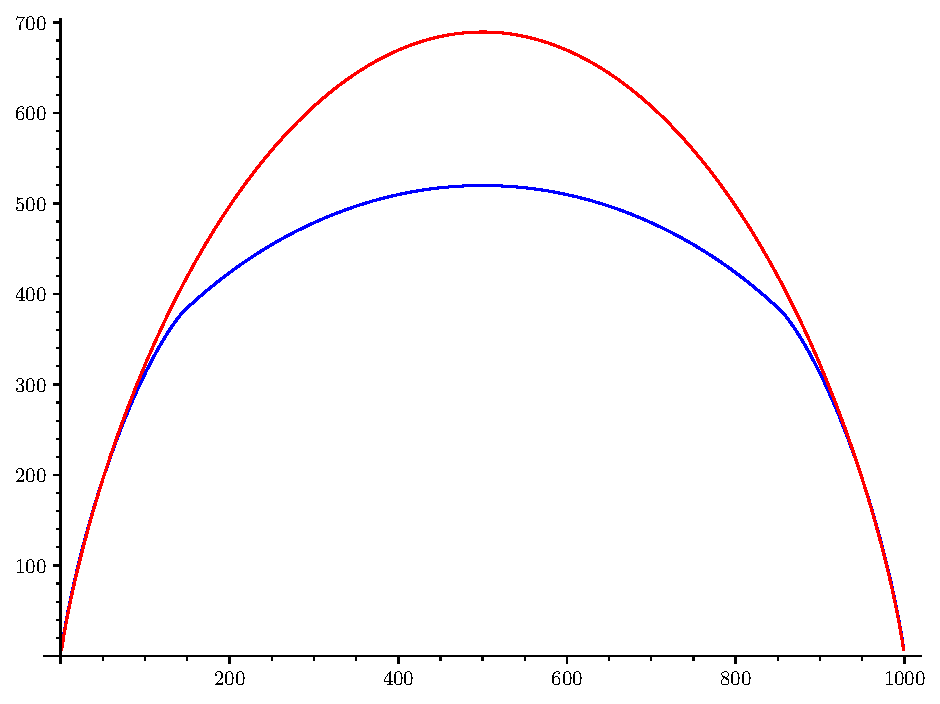
\includegraphics[width=7cm]{cauchy_estimate.pdf}
        \caption{Cauchy estimate in blue vs.\ binomial coefficients in red.}
        \label{fig:cauchy_estimate}
    \end{figure}
\end{remark}}




\subsection{Generalization to a family of weightwise quadratic functions}\label{sec:general}
In this part, we generalize the results of Section~\ref{sec:Cauchy} to all weightwise quadratic function such that for all $k\in [1,n]$, the function $f_k$ has exactly $t$ quadratic terms with no shared variables.




\begin{definition}
	Let $n\in \N^*$ be an even number and $t \in \N $ no greater than $n/2$, we denote by $d_{t,n}$ the function given by: $d_{t,n}(x)=\sum_{i=1}^t x_{2i-1} x_{2i}$.
	
	%	by $\Dnka{n}{k}{a}$:
	%	\[\Dnka{n}{k}{a}= \sum_{x\in \Ekn{k}{n}} (-1)^{d_n(x) +a x}\]
\end{definition}

In particular, $d_{\frac{n}{2},n}(x)=d_n(x)$. 
%We focus on the Walsh spectrum restricted to the slices of any function $d_{t,n}$:
We focus on the restricted Walsh spectrum of any function $d_{t,n}$:

\begin{proposition}\label{proposition:dtn}
	Let $t, n\in \N$ with $n$ even and $t\le n/2$, the following holds on $d_{t,n}$ for all $k\in [0,n]$:
	\[\wtk{d_{t,n}}{k}(a)=\sum_{\ell=0}^{2t} \Dnka{2t}{\ell}{b} \kraw{k-\ell}{\w(c)}{n-2t},\]
	where $b$ denotes the first $2t$ elements of $a$ and $c$ the last $n-2t$ elements.
\end{proposition}
\begin{proof}
	We rewrite the restricted Walsh transform, denoting $x\in \F_2^n$ by $(y,z)$ where $y\in \F_2^{2t}$ and $z \in \F_2^{n-2t}$, and similarly denoting $a$ by $(b,c)$:
	
%	\begin{align*}
%	\wtk{d_{t,n}}{k}(a)&=\sum_{x \in \Ekn{k}{n}} (-1)^{d_{t,n}(x)+ax}=\sum_{x \in \Ekn{k}{n}} (-1)^{d_{t,t}(y)+by +cz}\\
%	&=\sum_{\ell=0}^{2t} \sum_{\substack{y \in \Ekn{\ell}{2t}\\z \in \Ekn{k-\ell}{n-2t}}} (-1)^{d_{t,t}(y)+by +cz}\\
%	&=\sum_{\ell=0}^{2t} \sum_{y \in \Ekn{\ell}{2t}} (-1)^{d_{t,t}(y)+by} \left( \sum_{z \in \Ekn{k-\ell}{n-2t}} (-1)^{cz}\right)\\
%	&=\sum_{\ell=0}^{2t} \Dnka{2t}{\ell}{b} \kraw{k-\ell}{\w(c)}{n-2t}.%\qedhere
%	\end{align*}	

	\begin{align*}
\wtk{d_{t,n}}{k}(a)&=\sum_{x \in \Ekn{k}{n}} (-1)^{d_{t,n}(x)+a \cdot x}=\sum_{x \in \Ekn{k}{n}} (-1)^{d_{t,2t}(y)+b \cdot y +c \cdot z}=\sum_{\ell=0}^{2t} \sum_{\substack{y \in \Ekn{\ell}{2t}\\z \in \Ekn{k-\ell}{n-2t}}} (-1)^{d_{t,2t}(y)+b \cdot y +c \cdot z}\\
&=\sum_{\ell=0}^{2t} \sum_{y \in \Ekn{\ell}{2t}} (-1)^{d_{t,2t}(y)+b \cdot y} \left( \sum_{z \in \Ekn{k-\ell}{n-2t}} (-1)^{c \cdot z}\right)=\sum_{\ell=0}^{2t} \Dnka{2t}{\ell}{b} \kraw{k-\ell}{\w(c)}{n-2t}.\qedhere
\end{align*}	



\end{proof}

\begin{definition}\label{defi:P_a_t}
    Let $t, n\in \N$ with $n$ even and $t\le n/2$. Given $a=(b,c)\in\F_2^n$ with $b\in\F_2^{2t}$, denote $n-2t-\w(c)$ and $\w(c)$ by $u$ and $v$, respectively. We  then introduce the following polynomial:
    \[
        P_{a,t}(z)=P_b(z)\cdot(1+z)^u\cdot(1-z)^v.
    \]
\end{definition}

\begin{proposition}
    Let $t, n\in \N$ with $n$ even and $t\le n/2$. Let $a\in\F_2^n$. The following holds true: 
    \[
        \sum_{k\in\Z}\wtk{d_{t,n}}{k}(a)z^k=P_{a,t}(z).
    \]
\end{proposition}

\begin{proof}
    Applying Proposition \ref{proposition:dtn}, we get:
    \begin{align*}
        \sum_{k\in\Z}\wtk{d_{t,n}}{k}(a)z^k&=\sum_{\ell=0}^{2t}\Dnka{2t}{\ell}{b}z^\ell\sum_{k\in\Z}\kraw{k-\ell}{\w(c)}{n-2t}z^{k-\ell}\\
        &=\left(\sum_{\ell=0}^{2t}\Dnka{2t}{\ell}{b}z^\ell\right)\cdot(1+z)^u\cdot(1-z)^v\\
        &=P_b(z)\cdot(1+z)^u\cdot(1-z)^v\\
        &=P_{a,t}(z).\qedhere
    \end{align*}
\end{proof}

With this, we prove a generalization of Theorem~\ref{theorem:bound_D_nka} below. Before that, we still require a preliminary result:

\begin{lemma}\label{lemma:maximizing_args}
    Let $N$ be a non-negative number and $D\subseteq\C$ a set of complex numbers. For every integer $1\leq i\leq N$, consider a non-negative integer $m_i$ as well as complex functions $f_{i,1},\dots,f_{i,k_i}$ defined on the set $D$. Assume that the following maximum exists (which holds for instance if the functions $f_{i,j}$ are continuous and $D$ is topologically compact):
    \[
        M=\max_{\substack{\forall 1\leq i\leq N:\,p_{i,1}+\cdots+p_{i,k_i}=m_i\\z\in D}}\left|\prod_{i=1}^N\prod_{j=1}^{k_i}f_{i,j}(z)^{p_{i,j}}\right|.
    \]
    Then there exist integers $j_1,\dots,j_N$ with $1\leq j_i\leq k_i$ such that the following holds:
    \[
        M=\max_{z\in D}\left|\prod_{i=1}^Nf_{i,j_i}(z)^{m_i}\right|.
    \]
\end{lemma}

\begin{proof}
    Let us choose the integers $p_{i,j}$ and the complex number $z\in D$ to maximize the quantity $\left|\prod_{i=1}^N\prod_{j=1}^{k_i}f_{i,j}(z)^{p_{i,j}}\right|$. Note that this in particular means that $\sum_{j=1}^{k_i}p_{i,j}=m_i$ for every $1\leq i\leq N$. Next, for every $1\leq i\leq N$, choose $1\leq j_i\leq k_i$ such that $|f_{i,j_i}(z)|\geq|f_{i,j}(z)|$ for every $1\leq j\leq k_i$. Then we have:
    \[
        M=\left|\prod_{i=1}^N\prod_{j=1}^{k_i}f_{i,j}(z)^{p_{i,j}}\right|\leq\left|\prod_{i=1}^N\prod_{j=1}^{k_i}f_{i,j_i}(z)^{p_{i,j}}\right|=\left|\prod_{i=1}^Nf_{i,j_i}(z)^{\sum_{j=1}^{k_i}p_{i,j}}\right|=\left|\prod_{i=1}^Nf_{i,j}(z)^{m_i}\right|\leq M.\qedhere
    \]
\end{proof}

\begin{theorem}\label{theorem:bound_D_nka_generalized}
    Let $t, n\in \N$ with $n$ even and $t\le n/2$. 
    We define $\lambda=t/n\in\left[0,\frac 12\right]$, as well as:
    \[
        \mu(\lambda)=\mu=
        \begin{cases}
            \frac{\lambda+1}{2}+\frac12\log_2\left(\frac{\left(-\lambda^2+2\lambda+\lambda\sqrt{\lambda^2-4\lambda+2}\right)^\lambda}{\left(1-\lambda+\sqrt{\lambda^2-4\lambda+2}\right)^{2\lambda-1}}\right)&\text{if $\lambda>\frac 16$,}\\
            1-\lambda&\text{if $\lambda\leq\frac 16$.}\\
        \end{cases}
    \]

    Then, for all $a\in\F_2^n$ and $k\in[0,n]$, the following hold true:

    \[
        |\wtk{d_{t,n}}{k}(a)|\leq 2^{\mu n}\quad \text{and} \quad  |\wt{d_{t,n}}(a)|\leq 1+n\cdot 2^{\mu n}.
    \]
\end{theorem}

\begin{proof}
    To begin, we observe that the inequality $|\wt{d_{t,n}}(a)|\leq 1+n\cdot 2^{\mu n}$ will follow from the inequality $|\wtk{d_{t,n}}{k}(a)|\leq 2^{\mu n}$ using precisely the arguments of the proof of Corollary~\ref{cor:bound_walsh_cauchy}, so that we are only required to prove the first inequality. Also, since the case $\lambda=\frac 12$ corresponds to Theorem~\ref{theorem:bound_D_nka}, we will henceforth assume $\lambda<\frac 12$.
    
    As before in the proof of Theorem~\ref{theorem:bound_D_nka}, we want to bound the maximum of $|P_{a,t}(z)|$ on $\dis$ for $a\in\F_2^n$, and this will then be an upper bound on $|\wtk{d_{t,n}}{k}(a)|$ for every $k\in[1,n]$. 
    We write $a=(b,c)$ with $b\in\F_2^{2t}$ and define $(p,q,r)=(p(b),q(b),r(b))$, and further consider $u=n-2t-\w(c)$ and $v=\w(c)$ as in Definition~\ref{defi:P_a_t}.    
   To find a bound for $|P_{a,t}(z)|$ on $\dis$ that applies to all $a\in\F_2^n$, we would like to bound the quantity $\max_{a\in\F_2^n,z\in\dis}|P_{a,t}(z)|$. Moving through all $a\in\F_2^n$ is equivalent to moving through all tuples $(p,q,r;u,v)$ of non-negative integers which satisfy $p+q+r=t$ and $u+v=n-2t$. It follows from Lemma~\ref{lemma:maximizing_args} that it is enough to consider only the cases for which only one of $p,q,r$ is non-zero, and for which only one of $u,v$ is non-zero. 
   This leaves us with the following cases to consider for $(p,q,r;u,v)$:
    \begin{gather*}
        (t,0,0;n-2t,0),\quad(0,t,0;n-2t,0),\quad(0,0,t;n-2t,0),\\
         (t,0,0;0,n-2t),\quad(0,t,0;0,n-2t),\quad(0,0,t;0,n-2t).
    \end{gather*}
    Since swapping both $(p,q)$ and $(u,v)$ has the same effect as replacing $z$ by $-z$ in $P_{a,t}(z)$ and therefore does not change the maximum of $|P_{a,t}(z)|$ on $\dis$, we can further restrict ourselves to the following tuples for $(p,q,r;u,v)$:
    \[
        (t,0,0;n-2t,0),\quad(0,t,0;n-2t,0),\quad(0,0,t;n-2t,0).
    \]
    Let us start by bounding $|P_{a,t}(z)|$ on $\dis$ in case $(p,q,r;u,v)=(t,0,0;n-2t,0)$. Since $t=\lambda n$, we can write:
    \[
        P_{a,t}(z)=\left((-z^2+2z+1)^{\lambda}(1+z)^{1-2\lambda}\right)^n.
    \]
    Further writing $z=\ee^{\ii\alpha}$ and $z^2=\ee^{2\ii\alpha}$ for $\alpha\in[-\pi,\pi]$, and using that $|w|^2=w\overline w$ for every complex number $w$, we get:
    \begin{align*}
        |-z^2+2z+1|^2&=\left(-\ee^{2\ii\alpha}+2\ee^{\ii\alpha}+1\right)\left(-\ee^{-2\ii\alpha}+2\ee^{-\ii\alpha}+1\right)\\
        &=6-\ee^{2\ii\alpha}-\ee^{-2\ii\alpha}\\
        &=6-2\cos (2\alpha),
    \end{align*}
    where the last equality uses that $\ee^{2\ii\alpha}=\cos(2\alpha)+\ii\sin(2\alpha)$. We similarly obtain that $|1+z|^2=2+2\cos\alpha$. Combining both, we get:   
    \[
        |P_{a,t}(z)|^2=\left(\left|-z^2+2z+1\right|^{2\lambda}|1+z|^{2(1-2\lambda)}\right)^n=\left((6-2\cos(2\alpha))^\lambda(2+2\cos\alpha)^{1-2\lambda}\right)^n.
    \]
    
    The goal will be to prove that the maximum of $g_\lambda(\alpha)=g(\alpha)=(6-2\cos(2\alpha))^\lambda(2+2\cos\alpha)^{1-2\lambda}$ for $\alpha\in[-\pi,\pi]$ is equal to $2^{2\mu}$; the maximum of $|P_{a,t}(z)|$ on $\dis$ will then be $\left(2^{2\mu}\right)^{n/2}=2^{\mu n}$. Since $g$ is an even function, it is enough to focus on the interval $\alpha\in[0,\pi]$; the function $g$ is represented for several different values of $0\leq\lambda<\frac 12$ in Figure~\ref{fig:family_curves_g}.

    \begin{figure}
    	\centering
    	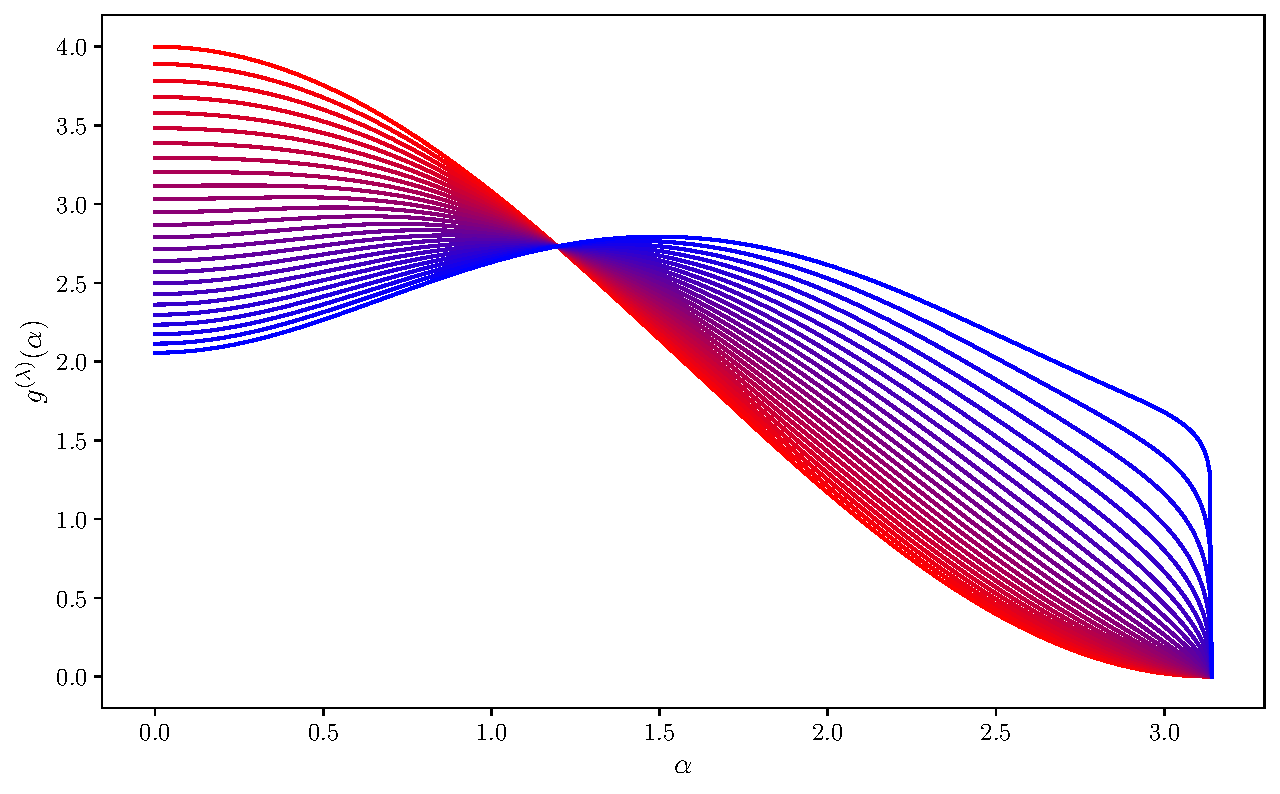
\includegraphics[width=11cm]{family_curves_g.pdf}
    	\caption{The curves of $\alpha\mapsto g_\lambda(\alpha)$ for the values $\lambda=\frac{i}{25}$ from $i=0$ (blue) to $i=24$ (red).}
    	\label{fig:family_curves_g}
    \end{figure}
    
    Writing $g(\alpha)=g_1(\alpha)^{\lambda}g_2(\alpha)^{1-2\lambda}$ for $g_1(\alpha)=6-2\cos(2\alpha)$ and $g_2(\alpha)=2+2\cos\alpha$, we compute the first derivative of $g$, and apply the double angle formulas $\cos(2\alpha)=2\cos^2\alpha-1$ and $\sin(2\alpha)=2\cos\alpha\sin\alpha$:
    \begin{align*}
         \frac{\dd}{\dd\alpha}g(\alpha)&=g_1(\alpha)^{\lambda-1}g_2(\alpha)^{-2\lambda}\left(\lambda g_2(\alpha)\frac{\dd}{\dd\alpha}g_1(\alpha)+(1-2\lambda)g_1(\alpha)\frac{\dd}{\dd\alpha}g_2(\alpha)\right)\\
         &=g_1(\alpha)^{\lambda-1}g_2(\alpha)^{-2\lambda}\left(\lambda(2+2\cos\alpha)\cdot4\sin(2\alpha)+(1-2\lambda)(6-2\cos(2\alpha))(-2\sin\alpha)\right)\\
         &=g_1(\alpha)^{\lambda-1}g_2(\alpha)^{-2\lambda}\left(\lambda(2+2\cos\alpha)\cdot4\cdot2\cos\alpha\sin\alpha+(1-2\lambda)\left(8-4\cos^2\alpha\right)(-2\sin\alpha)\right)\\
         &=8g_1(\alpha)^{\lambda-1}g_2(\alpha)^{-2\lambda}\sin\alpha\left(2\lambda \cos\alpha(1+\cos\alpha)-(1-2\lambda)\left(2-\cos^2\alpha\right)\right)\\
         &=8g_1(\alpha)^{\lambda-1}g_2(\alpha)^{-2\lambda}\sin\alpha\left(\cos^2\alpha+2\lambda\cos\alpha+4\lambda-2\right).
    \end{align*}
    
    The only interesting zeros of $\frac{\dd}{\dd\alpha}g(\alpha)$ are those of the last factor 
    $\cos^2\alpha+2\lambda\cos\alpha+4\lambda-2$: those of the factor $8(6-2\cos(2\alpha))^{\lambda-1}(2+2\cos\alpha)^{-2\lambda}$ will make $g(\alpha)$ vanish and will therefore not maximize $g(\alpha)$, and those for $\sin\alpha$ are $\alpha=0$ and $\alpha=\pi$, with corresponding values $g(0)=2^{2-2\lambda}$ and $g(\pi)=0$.
    
    Our first claim is that the equation $\mathcal E:\cos^2\alpha+2\lambda\cos\alpha+4\lambda-2=0$ has a unique solution $\cos\alpha=-\lambda+\sqrt{\lambda^2-4\lambda+2}$ if $\lambda\geq\frac 16$ and has no solution $\cos\alpha$ otherwise. To see this, we consider $\mathcal E$ as an equation of second degree in $\cos\alpha$, which leads to the two solution candidates $\cos\alpha=-\lambda\pm\sqrt{\lambda^2-4\lambda+2}$.
     
    We can exclude the solution $\cos\alpha=-\lambda-\sqrt{\lambda^2-4\lambda+2}$ since $\cos\alpha\in[-1,1]$. The other solution needs to be excluded for the same reason if $\lambda<\frac 16$.


    Our next claim is that $\frac{\dd^2}{\dd^2\alpha}g(\alpha)\vert_{\alpha=0}$ has the same sign as $6\lambda -1$. To see why, we apply the definition of the second derivative:
    \begin{align*}
        \frac{\dd^2}{\dd^2\alpha}g(\alpha)\vert_{\alpha=0}
        &=\lim_{\alpha\to 0}\frac{\frac{\dd}{\dd\alpha}g(\alpha)}{\alpha}\\
        &=\lim_{\alpha\to 0}8(6-2\cos(2\alpha))^{\lambda-1}(2+2\cos\alpha)^{-2\lambda}\cdot\frac{\sin\alpha}{\alpha}\cdot\left(\cos^2\alpha+2\lambda\cos\alpha+4\lambda-2\right)\\
        &=8\cdot4^{\lambda-1}\cdot 4^{-2\lambda}\cdot 1\cdot(6\lambda -1)\\
        &=2^{1-2\lambda}(6\lambda -1).
    \end{align*}


    Therefore, in case $\lambda<\frac 16$, we can conclude from the two claims that $g(\alpha)$ reaches its maximum at $\alpha_0=0$, and this maximum is then equal to $2^{2-2\lambda}=2^{2\mu}$, as required. For $\lambda=\frac 16$, the solution to the equation $\mathcal E$ is $\cos\alpha=1$, again implying that $g(\alpha)$ reaches its maximum at $\alpha_0=0$, and we obtain the same maximum of $2^{2\mu}$. In case $\lambda>\frac 16$, the two claims imply that $g(\alpha)$ reaches its maximum at the two values $\alpha_0\in[0,\pi]$ for which $\cos\alpha_0=-\lambda+\sqrt{\lambda^2-4\lambda+2}$. For such $\alpha_0$, the double angle formula for the cosine implies that $\cos(2\alpha_0)=2\lambda^2-4\lambda+2-2\lambda\sqrt{\lambda^2-4\lambda+2}$. If we replace $\cos\alpha_0$ and $\cos(2\alpha_0)$ by their respective values, we obtain that the maximum of $g(\alpha)$ for $\alpha\in[0,\pi]$ is given by the following value:

    \[
        g(\alpha_0)=\frac{\left(-8\lambda^2+16\lambda+8\lambda\sqrt{\lambda^2-4\lambda+2}\right)^{\lambda}}{\left(2-2\lambda+2\sqrt{\lambda^2-4\lambda+2}\right)^{2\lambda-1}}=2^{2\mu}.
    \]
    This is exactly what we wanted to prove, and we have therefore covered the case $(p,q,r;u,v)=(t,0,0;n-2t,0)$ entirely. In a similar fashion, it can be proven that $|P_{a,t}(z)|$ is also bounded by $2^{\mu n}$ on $\dis$ for the remaining two cases of $(p,q,r;u,v)$. In fact, for $(p,q,r;u,v)=(0,t,0;n-2t,0)$, it is enough to replace $g(\alpha)$ by $h_1(\alpha)=(6-2\cos(2\alpha))^\lambda(2-2\cos\alpha)^{1-2\lambda}$, which has the same maximum as $g(\alpha)$ because $h_1\left(\frac{\pi}{2}+\alpha\right)=g\left(\frac{\pi}{2}-\alpha\right)$; for $(p,q,r;u,v)=(0,0,t;n-2t,0)$, it is enough to replace $g(\alpha)$ by $h_2(\alpha)=(2+2\cos(2\alpha))^\lambda(2+2\cos\alpha)^{1-2\lambda}$, whose maximum is bounded by the maximum of $g(\alpha)$ because $h_2(\alpha)\leq g(\alpha)$.
\end{proof}

The curve of $\lambda\mapsto\mu(\lambda)$ defined in the above Theorem~\ref{theorem:bound_D_nka_generalized} is represented in Figure~\ref{fig:curve_exponents_lambda_mu}.

\begin{figure}
	\centering
	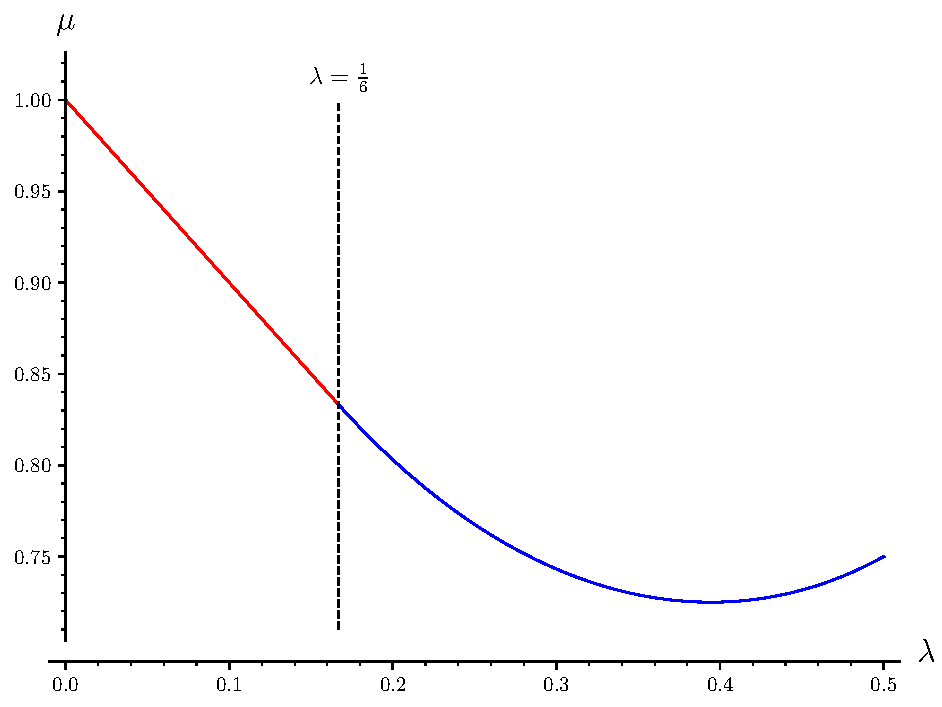
\includegraphics[width=10cm]{curve_exponents_lambda_mu.pdf}
	\caption{The curve of $\lambda\mapsto\mu(\lambda)$ with $0\leq\lambda\leq\frac 12$ from Theorem~\ref{theorem:bound_D_nka_generalized}.}
	\label{fig:curve_exponents_lambda_mu}
\end{figure}


%\pmnote{for the remark, add how they are obtained (from a script in xxx). 
%We can give the scripts in supplementary material when submitting, of add the link of a github if you agree to have them public. \color{blue} Tim: I added the script to GitHub. You can decide what we do with it.}

\section{Experiments and comparisons}

In this section, we establish a tighter bound on the absolute value of the Walsh transform of the revised HWBF for values of $n$ up to $80$. 
We then compare the nonlinearity of this function to that of other functions suited to similar use cases, such as the HWBF of weightwise cyclic functions from~\cite{DAM:MeaOza24}.

\subsection{Bounding the Walsh transform of $f$ experimentally}\label{sec:expwt}

%We have just deduced that $|\wt f(a)|\leq 1+n\cdot 2^{3n/4}$ for every Boolean vector $a\in\F_2^n$. This is a pessimistic bound. In this section, we will discuss how a tighter bound on $|\wt f(a)|$ can be obtained in polynomial time in $n$.

Following Corollary~\ref{cor:bound_walsh_cauchy} we deduce that $|\wt f(a)|\leq 1+n\cdot 2^{3n/4}$ for every Boolean vector $a\in\F_2^n$. This is a pessimistic bound. In this part, we discuss how a tighter bound on $|\wt f(a)|$ can be obtained in polynomial time in $n$.

%This method is based on the identity (\ref{eqn:walsh_from_D}). 
This method is based on the identity given in Proposition~\ref{prop:WT}.
For this, consider a vector $b\in\mathbb F_2^n$; we write $(p,q,r)=(p(b),q(b),r(b))$. Also, for $1\leq k\leq n$, let $b_k=b+\pi(e_k)$ and $(p_k,q_k,r_k)=(p(b_k),q(b_k),r(b_k))$. Observe that for every $1\leq k\leq n$, we have $(p_k,q_k,r_k)\in\{(p\pm1,q,r\mp 1),(p,q\pm 1,r\mp 1)\}$. Furthermore, observe that if $k\leq n/2$ and $(p_k,q_k,r_k)=(p+\alpha,q+\beta,r+\gamma)$ for $\{\alpha,\beta,\gamma\}=\{0,\pm 1\}$ with $\gamma\neq 0$, then we have $(p_{k+n/2},q_{k+n/2},r_{k+n/2})=(p+\alpha',q+\beta',r+\gamma')$ for some $\{\alpha',\beta',\gamma'\}=\{0,\pm 1\}$ with $\gamma'\neq 0$ which only depend on $\alpha$, $\beta$ and $\gamma$. Explicitly, we have $(\alpha',\beta',\gamma')=(\alpha,\beta,\gamma)$ if $\gamma=1$ and $(\alpha',\beta',\gamma')=(\beta,\alpha,\gamma)$ if $\gamma=-1$.

In the following discussion, we outline a method to determine an upper bound on $\max_{a\in\F_2^n}\wt f(a)$. A similar approach can be applied to find a lower bound on $\min_{a\in\F_2^n}\wt f(a)$, and by utilizing both, we can also obtain an upper bound on $\max_{a\in\F_2^n}|\wt f(a)|$ by making use of the following identity:
\[
\max_{a\in\F_2^n}|\wt f(a)|=\max\Big(\max_{a\in\F_2^n}\wt f(a),-\min_{a\in\F_2^n}\wt f(a)\Big).
\]
For each $1\leq k\leq n/2$, we select $\{\alpha_k,\beta_k,\gamma_k\}=\{0,\pm 1\}$ with $\gamma_k\neq 0$ such that the following expression is defined and maximized:
\[
B_k^{p,q,r}=\mathsf D_{n,k}^{p+\alpha_k,q+\beta_k,r+\gamma_k}+\mathsf D_{n,k+n/2}^{p+\alpha_k',q+\beta_k',r+\gamma_k'}.
\]
This implies that $\Dnka{n}{k}{b_k}+\Dnka{n}{k+n/2}{b_{k+n/2}}\leq B_k^{p,q,r}$ for every $1\leq k\leq n/2$, leading to the conclusion that $\sum_{k=1}^n\Dnka nk{b_k}\leq\sum_{k=1}^{n/2} B_k^{p,q,r}$. As a result, we derive the following upper bound:
\begin{equation}\label{eqn:bound_walsh}
\max_{a\in\F_2^n}\wt f(a)\leq\max_{p+q+r=n/2}\sum_{k=1}^{n/2} B_k^{p,q,r}.
\end{equation}
Under the assumption that the values of $\mathsf{D}_{n,k}^{p,q,r}$ have already been computed for all triplets $(p,q,r)$ satisfying $p+q+r=n/2$, the bound in equation (\ref{eqn:bound_walsh}) can be determined with a computational complexity of $\mathcal{O}(n^3)$. This is because there are $\mathcal{O}(n^2)$ possible triplets $(p,q,r)$ that meet the condition $p+q+r=n/2$, and the summation itself can be computed in $\mathcal{O}(n)$.

We consider now the complexity involved in computing the values of $\mathsf{D}_{n,k}^{p,q,r}$ for all $0 \leq k \leq n$ and for all triplets $(p,q,r)$ where $p+q+r=n/2$. We claim that this computation has a complexity of $\mathcal{O}(n^3 \log n)$. Towards this, according to Proposition \ref{proposition:generating_fct}, it is sufficient to expand the polynomials $(-z^2 + 2z + 1)^p \cdot (-z^2 - 2z + 1)^q \cdot (z^2 + 1)^r$ for all triplets $(p,q,r)$ such that $p+q+r=n/2$.

To achieve this, we first precompute the expanded polynomials $(-z^2 + 2z + 1)^p$ for each $1 \leq p \leq n/2$. This can be done recursively using the formula $(-z^2 + 2z + 1)^{p+1} = (-z^2 + 2z + 1) \cdot (-z^2 + 2z + 1)^p$. For each $p$, we need to compute the product of two expanded polynomials of degree at most $n/2$, which requires $\mathcal{O}(n \log n)$ computations . Performing this for every $p$ results in a total complexity of $\mathcal{O}(n^2 \log n)$. The same approach is used to expand the polynomials $(-z^2 - 2z + 1)^q$ and $(z^2 + 1)^r$, resulting in an overall complexity of $\mathcal{O}(n^2 \log n)$ for this precomputational step.

Finally, for each triplet $(p,q,r)$ where $p+q+r=n/2$, we multiply the expanded polynomials $(-z^2 + 2z + 1)^p$, $(-z^2 - 2z + 1)^q$, and $(z^2 + 1)^r$. These two multiplications are once more performed in $\mathcal{O}(n \log n)$. Given that there are $\mathcal{O}(n^2)$ such triplets $(p,q,r)$, the complexity of this step totals $\mathcal{O}(n^3 \log n)$. Therefore, this final step is the primary computational bottleneck, making the overall complexity of the procedure also $\mathcal{O}(n^3 \log n)$.



\pmnote{add a link to the public github or name of the name of this code in supplementary materials.}

\tsnote{Is on GitHub now: \texttt{Bounding\_Walsh.ipynb}}


%Table~\ref{table:max_walsh_vs_bound} compares $\max_{a\in\mathbb F_2^n}|\wt f(a)|$ to the upper bound $B_n$ we find using the above method. Table~\ref{table:walsh_bounds} gives all values of this bound $B_n$ for all even $1\leq n\leq 80$.

In Table~\ref{table:max_walsh_vs_bound}, we compare the exact values of $\max_{a\in\mathbb F_2^n}|\wt f(a)|$ for small values of $n$ (calculated using \textsf{SageMath}) to the upper bound $B_n$ obtained through the above method and the one from Corollary~\ref{cor:bound_walsh_cauchy}. 
Additionally, Table~\ref{table:walsh_bounds} provides the values of the bound $B_n$ for all even values of $n$ from $1$ to $80$.
We observe that the above method provides a much tighter bound than the one from Corollary~\ref{cor:bound_walsh_cauchy}, and its polynomial complexity enables us to extend the analysis far beyond what is feasible with a full computation of the Walsh spectrum (\( \mathcal{O}(n 2^n) \)).



\iffalse
\begin{table}
	\centering
	\begin{tabular}{|c|c|c|}
		\hline
		$n$ & $\max_{a\in\F_2^n}|W_f(a)|$ & $B_n$ \\ \hline
		$2$  & $2$     & $4$     \\
		$4$  & $8$     & $14$     \\
		$6$  & $20$    & $36$    \\
		$8$  & $52$    & $114$    \\
		$10$ & $108$   & $288$   \\
		$12$ & $292$   & $820$   \\
		$14$ & $700$   & $2\,316$  \\
		$16$ & $2\,176$  & $6\,006$  \\
		$18$ & $4\,964$  & $18\,192$  \\
		$20$ & $14\,968$ & $48\,480$ \\
		$22$ & $34\,232$ & $140\,392$ \\
		$24$ & $109\,648$ & $392\,168$ \\ \hline
	\end{tabular}
	\tablecaption{The actual $\max_{a\in\F_2^n}|W_f(a)|$ compared to the bound $B_n$}
	\label{table:max_walsh_vs_bound}
\end{table}
\fi



\begin{table}
	\centering
	\begin{tabular}{|c|c|c|c|}
		\hline
		$n$ & $\max_{a\in\F_2^n}|W_f(a)|$ & $B_n$  & $\lfloor 1+n \cdot 2^{3n/4} \rfloor$\\ \hline
		$2$  & $2$     & $4$  &  $6$ \\
		$4$  & $8$     & $14$  & $33$  \\
		$6$  & $20$    & $36$   & $136$\\
		$8$  & $52$    & $114$  & $513$ \\
		$10$ & $108$   & $288$  & $1\,811$\\
		$12$ & $292$   & $820$  & $6\,145$ \\
		$14$ & $700$   & $2\,316$ & $20\,275$ \\
		$16$ & $2\,176$  & $6\,006$ & $65\,637$ \\
		$18$ & $4\,964$  & $18\,192$ & $208\,535$ \\
		$20$ & $14\,968$ & $48\,480$ & $655\,361$ \\
		$22$ & $34\,232$ & $140\,392$ & $2\,039 \,002$ \\
		$24$ & $109\,648$ & $392\,168$ & $6\,291 \,457$  \\ \hline
	\end{tabular}
	\tablecaption{The actual $\max_{a\in\F_2^n}|W_f(a)|$ compared to the bound $B_n$ and the one from Corollary~\ref{cor:bound_walsh_cauchy}.}
	\label{table:max_walsh_vs_bound}
\end{table}



\begin{table}
	\centering
	\begin{minipage}{0.24\textwidth}
		\centering
		\begin{tabular}{|c|c|}
			\hline
			$n$ & $\approx B_n$ \\
			\hline
			$2$  & $4.00 \cdot 10^{0}$  \\
			$4$  & $1.40 \cdot 10^{1}$  \\
			$6$  & $3.60 \cdot 10^{1}$  \\
			$8$  & $1.14 \cdot 10^{2}$  \\
			$10$ & $2.88 \cdot 10^{2}$  \\
			$12$ & $8.20 \cdot 10^{2}$  \\
			$14$ & $2.32 \cdot 10^{3}$  \\
			$16$ & $6.01 \cdot 10^{3}$  \\
			$18$ & $1.82 \cdot 10^{4}$  \\
			$20$ & $4.85 \cdot 10^{4}$  \\
			\hline
		\end{tabular}
	\end{minipage}%
	\begin{minipage}{0.24\textwidth}
		\centering
		\begin{tabular}{|c|c|}
			\hline
			$n$ & $\approx B_n$ \\
			\hline
			$22$ & $1.40 \cdot 10^{5}$  \\
			$24$ & $3.92 \cdot 10^{5}$  \\
			$26$ & $1.14 \cdot 10^{6}$  \\
			$28$ & $3.12 \cdot 10^{6}$  \\
			$30$ & $8.90 \cdot 10^{6}$  \\
			$32$ & $2.50 \cdot 10^{7}$  \\
			$34$ & $7.14 \cdot 10^{7}$  \\
			$36$ & $2.04 \cdot 10^{8}$  \\
			$38$ & $5.75 \cdot 10^{8}$  \\
			$40$ & $1.62 \cdot 10^{9}$  \\
			\hline
		\end{tabular}
	\end{minipage}%
	\begin{minipage}{0.24\textwidth}
		\centering
		\begin{tabular}{|c|c|}
			\hline
			$n$ & $\approx B_n$ \\
			\hline
			$42$ & $4.59 \cdot 10^{9}$  \\
			$44$ & $1.29 \cdot 10^{10}$ \\
			$46$ & $3.63 \cdot 10^{10}$ \\
			$48$ & $1.02 \cdot 10^{11}$ \\
			$50$ & $2.88 \cdot 10^{11}$ \\
			$52$ & $8.06 \cdot 10^{11}$ \\
			$54$ & $2.30 \cdot 10^{12}$ \\
			$56$ & $6.45 \cdot 10^{12}$ \\
			$58$ & $1.83 \cdot 10^{13}$ \\
			$60$ & $5.14 \cdot 10^{13}$ \\
			\hline
		\end{tabular}
	\end{minipage}%
	\begin{minipage}{0.24\textwidth}
		\centering
		\begin{tabular}{|c|c|}
			\hline
			$n$ & $\approx B_n$ \\
			\hline
			$62$ & $1.47 \cdot 10^{14}$ \\
			$64$ & $4.09 \cdot 10^{14}$ \\
			$66$ & $1.17 \cdot 10^{15}$ \\
			$68$ & $3.25 \cdot 10^{15}$ \\
			$70$ & $9.34 \cdot 10^{15}$ \\
			$72$ & $2.60 \cdot 10^{16}$ \\
			$74$ & $7.44 \cdot 10^{16}$ \\
			$76$ & $2.08 \cdot 10^{17}$ \\
			$78$ & $5.97 \cdot 10^{17}$ \\
			$80$ & $1.65 \cdot 10^{18}$ \\
			\hline
		\end{tabular}
	\end{minipage}
	\tablecaption{Approximate values of $B_n$ for various values of $n$}
	\label{table:walsh_bounds}
\end{table}



\subsection{Comparison of the nonlinearity}

\pmnote{under construction}

In this part we compare the nonlinearity of the function $f$ from Definition~\ref{def:revHWBF} to other weightwise quadratic functions considered for similar use-cases, such as majority, HWBF and the cyclic weighwise functions studied in~\cite{DAM:MeaOza24}. 


%In Figure~\ref{fig:walsh_bound_comparison} we compare the value $\max_{a\in\mathbb F_2^n}|\wt f(a)|$, the smaller the maximum the better the nonlinearity. We display the values for $n$ up to $80$, which is sufficient to compare the asymptotic behavior of the different bounds. 
%The violet and orange curves correspond to the upper bounds proven in~\cite{DAM:MeaOza24}. The violet one corresponds to the bound holding for all cyclic weightwise linear function such that $f_0(x)=b\cdot x$ with $\w(b)$ odd. It gives for example an upper bound for the HWBF. The orange one corresponds to the bound holding the cyclic weightwise quadratic function given by $f_0(x)=x_1+x_2x_3$. 
%The blue curve corresponds to both the majority and HWBF function, whose exact nonlinearity are recalled in Property~\ref{prop:wwd1}. We use only one curve since on a logarithmic scale the difference of nonlinearity between these two functions is too small to differentiate the curves. 
%Regarding the revisited HWBF introduced in Definition~\ref{def:revHWBF}, the red curve corresponds to the theoretical bound from Corollary~\ref{cor:bound_walsh_cauchy}, and the green one the experimental approach of Section~\ref{sec:expwt}.

In Figure~\ref{fig:walsh_bound_comparison}, we compare the values of $\max_{a \in \mathbb{F}_2^n} |\wt f(a)|$, where a smaller maximum indicates better nonlinearity (see Definition~\ref{def:nl}). 
We present values for $n$ up to $80$, which is sufficient for examining the asymptotic behavior of the different bounds.
The violet and orange curves represent the upper bounds  in~\cite{DAM:MeaOza24}. The violet curve corresponds to the bound that holds for all cyclic weightwise linear functions where $ f_0(x) = b \cdot x $ with $\w(b)$ odd, providing, for example, an upper bound for the HWBF. The orange curve corresponds to the bound for the cyclic weightwise quadratic function defined by $f_0(x) = x_1 + x_2 x_3$.
The blue curve represents both the majority and HWBF functions, whose exact nonlinearities are given in Property~\ref{prop:wwd1}. We use a single curve here because, on a logarithmic scale, the nonlinearity difference between these two functions is too small to distinguish between them.
For the revisited HWBF introduced in Definition~\ref{def:revHWBF}, the red curve corresponds to the theoretical bound from Corollary~\ref{cor:bound_walsh_cauchy}, while the green curve represents the experimental results from Section~\ref{sec:expwt}.

\begin{figure}
	\centering
	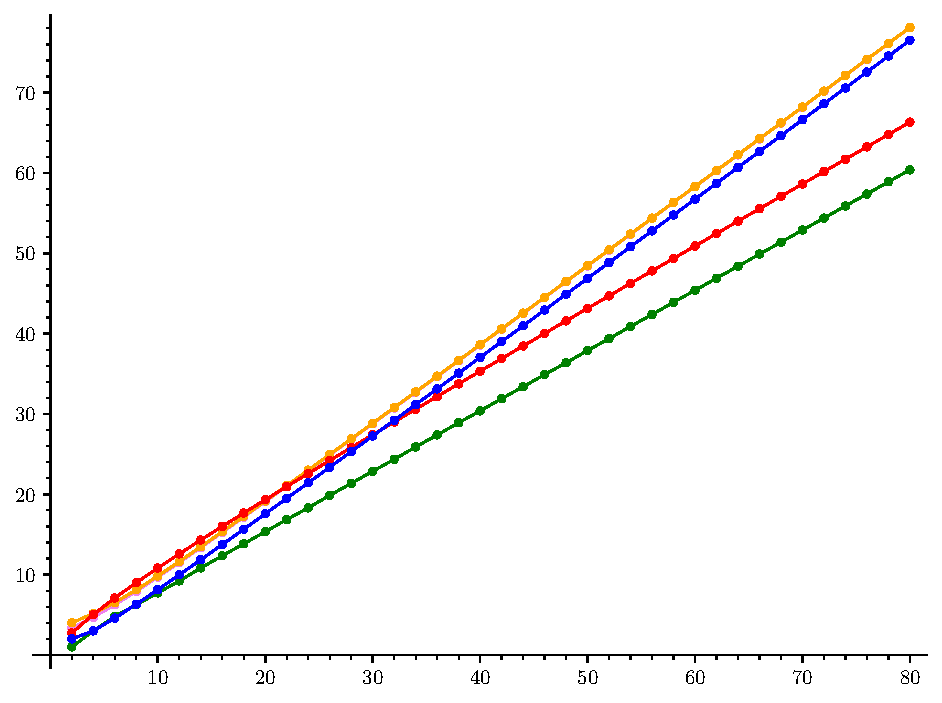
\includegraphics[width=9cm]{comparison_walsh_bound.pdf}
	\caption{
		%Maximum of the absolute value of the Walsh spectrum of different functions, in logarithmic scale, for even values of $n$. In violet and orange are the bounds for the cyclic weigtwise linear functions and one cyclic weightwise quadratic function from~\cite{DAM:MeaOza24}. In blue is the value for the majority function and HWBF. The theoretical bound (Corollary~\ref{cor:bound_walsh_cauchy}) for the function $f$ is in red and the experimental one $B_n$ (Section~\ref{sec:expwt}) is in green.}		
		%On a logarithmic scale, our experimental bound $B_n$ in terms of $n$ in red, our theoretical bound $1+n\cdot 2^{3n/4}$ from Proposition \ref{cor:bound_walsh_cauchy} in green, and the bound $\binom{n}{n/2}$ in blue. \tsnote{Updated plot, but the description now needs to be changed.}}
		Maximum absolute values of the Walsh spectrum for various functions, shown on a logarithmic scale for even values of $n$. 
		The violet and orange curves represent bounds for cyclic weightwise linear functions and a cyclic weightwise quadratic function from~\cite{DAM:MeaOza24}. The blue curve shows values for the majority function and HWBF. The theoretical bound for the function $f$ (from Corollary~\ref{cor:bound_walsh_cauchy}) is in red, and the experimental bound $B_n$ (Section~\ref{sec:expwt}) is in green.}
	\label{fig:walsh_bound_comparison}
\end{figure}



We observe significantly better performance for the newly introduced function $f$ compared to the majority function and HWBF, with the proven bound exhibiting an asymptotic slope of $ 3/4$ as opposed to $1$. The two bounds proven in~\cite{DAM:MeaOza24} also have an asymptotic slope of $1$.
The gap between the red and green curves, both representing upper bounds on $ \max_{a \in \mathbb{F}_2^n} |\wt f(a)| $ (with only the formula for the red curve proven for all even $n$), suggests that the true values may follow an even better slope than $ 3/4$.

In Table~\ref{table:comparisonsNL}, we compare the specific nonlinearity values of the functions under consideration. Among the various weightwise quadratic functions studied so far, we observe that $f$ has the highest nonlinearity from $n=10$ onward.



\begin{table}[h]
	\centering
	\begin{tabular}{|c| c|c|c|c| c|c|c|}
		\hline
		$n$ & $4$  & $6$  & $8$  &  $10$ & $12$ & $14$ & $16$  \\
	\hline	
    	HWBF   & $4$  & $20$  & $88$  &  $372$ & $1544$ & $6344$ & $25904$  \\  	
   %4 10 20 44 88 186 372 772 1544 3172 6344 12952 25904
		\hline
Majority   & $5$  & $22$  & $93$  &  $386$ & $1586$ & $6476$ & $26333$  \\
\hline
		%cyclic $f_0=x_1+x_2x_3$
    	t~\cite{DAM:MeaOza24}   & $4$  & $22$  & $96$  &  $404$ & $1672$ & $6854$ & $27884$\\
    	%4 10 22 46 96 196 404 816 1672 3358 6854 13722 27884
\hline	
%$f_0= x_1 + \sum_{i=1}^{n/2-1}x_{2i}x_{2i+1}$	
    	u~\cite{DAM:MeaOza24}   & $4$  & $24$  & $104$  &  $456$ & $1888$ & $7816$ & $31616$ \\
    	%4 10 24 48 104 220 456 924 1888 3862 7816 15748 31616
\hline				
		
		$f$  & $4$  & $22$  & $102$  &  $458$ & $1902$ & $7842$ & $31680$\\
\hline
	\end{tabular}
	\caption{Comparison of the nonlinearity.}
	\label{table:comparisonsNL}
\end{table}





\section{Other parameters}
\subsection{Algebraic immunity of $f$}

\begin{proposition}[Algebraic immunity of $f$]
	Let $n\in \N$ be even, $f$ defined as
	$f(x_1,\cdots,x_n)=\left(\sum_{i=1}^{n/2} (x_i+1) x_{i+\frac{n}{2}}\right) + \sum_{k=1}^n \phikn{k}{n} x_k$ and $h$ denote the $n$-variable HWBF, the following holds:
	\[\AI(f)\ge \AI(h)-2.\]
\end{proposition}
\begin{proof}
	Let denote by $q$ the quadratic function $\sum_{i=1}^{n/2} (x_i+1) x_{i+\frac{n}{2}}$, it allows to write $h=f+q$. 
	Let $g\neq 0$ be an annihilator of $f+ \varepsilon$ of minimum degree (where $\varepsilon \in \{0,1\}$), then the following holds:
	\[g (1+q) (h+\varepsilon) = g(1+q) (f+\varepsilon + q)=0, \]
	hence $g (1+q)$ is an annihilator of $h+ \varepsilon$. 
	If $g (1+q)\ne 0$ then $\degg(g(1+q)) \le \degg(g)+2$ and we obtain $\degg(g)\ge \AI(h) -2$. 
	Otherwise, $g (1+q)= 0$ implies that $g$ annihilates $1+q$ and therefore $0=g (f+\varepsilon + 1 +q)=g(h+ \varepsilon +1)$ that is $\degg(g)\ge \AI(h)$. 
	Summarizing, for any non null annihilator $g$ of $f$ or $f+1$ we get $\degg(g)\ge \AI(h)-2$, it allows to conclude $\AI(f)\ge \AI(h)-2$.
\end{proof}

From~\cite{DAM:WCST14} Theorem 4, the algebraic immunity of the HWBF is at least $\lfloor n/3\rfloor +1$, which leads to $\lfloor n/3\rfloor -1$ for $f$.



\newpage

%%%%%%%%%%%%%%%%%%%%%%%%%%%%%%%%%%%%%%%


\ifnum\full=0
%%%%%%%%%%%%%%%%%%%%%%%%%%%%%%%%%%%%%%%%%%%%
\bibliographystyle{splncs04}
\bibliography{add}
%%%%%%%%%%%%%%%%%%%%%%%%%%%%%%%%%%%%%%%%%%%%
\else
%%%%%%%%%%%%%%%%%%%%%%%%%%%%%%%%%%%%%%%%%%%%
\bibliographystyle{alpha}
\bibliography{add}
%%%%%%%%%%%%%%%%%%%%%%%%%%%%%%%%%%%%%%%%%%%%
\fi

\end{document}
